\documentclass[a4paper,12pt]{article}
\usepackage[utf8]{inputenc}
\usepackage[ngerman]{babel}
\usepackage{amsmath}
\usepackage{amssymb}
\usepackage{amsthm}
\usepackage{geometry}
\usepackage{graphicx}
\usepackage[hidelinks]{hyperref}
\usepackage{xcolor}
\usepackage{enumitem}
\usepackage{booktabs}
\usepackage{array}
\usepackage[protrusion=true,expansion=true,final]{microtype}

\geometry{margin=2.5cm}
\tolerance=2000
\emergencystretch=3em
\hfuzz=0.5pt
\vfuzz=0.5pt

\renewcommand{\qedsymbol}{$\blacksquare$}

\theoremstyle{plain}
\newtheorem{satz}{Satz}
\newtheorem{lemma}{Lemma}
\newtheorem{korollar}{Korollar}
\theoremstyle{definition}
\newtheorem{definition}{Definition}
\newtheorem{beispiel}{Beispiel}
\theoremstyle{remark}
\newtheorem{bemerkung}{Bemerkung}

\setlist[itemize,1]{label=--}
\definecolor{mainblue}{RGB}{25,70,140}
\definecolor{accentred}{RGB}{180,50,30}
\hypersetup{colorlinks=true,linkcolor=mainblue,
            citecolor=accentred,urlcolor=mainblue}

\newcommand{\Gbio}{G_{\mathrm{bio}}}
\newcommand{\Gppi}{G_{\mathrm{PPI}}}
\newcommand{\Ggen}{G_{\mathrm{Gen}}}
\newcommand{\Gepi}{G_{\mathrm{Epi}}}
\newcommand{\Gkrebs}{G_{\mathrm{Krebs}}}
\newcommand{\Gblood}{G_{\mathrm{blood}}}
\newcommand{\sigvec}{\vec{\sigma}}

\title{Bioinformatik-Synthese: Einheitlicher\\
Graphen-Rahmen f\"ur biologische Netzwerke\\[6pt]
PPI, Genomnetzwerke, Epidemie-Ausbreitung\\
und Cancer-Graph-Theorie via Subgraph-Isomorphie}
\author{Stephan Epp\\[4pt]
\small Universit\"at Bielefeld}
\date{8.\ Juni 2026}

\begin{document}
\maketitle

\begin{abstract}
Diese Arbeit entwickelt einen \emph{universellen graphentheoretischen Rahmen}
$\Gbio = (V, E, w)$ f\"ur biologische Netzwerke und beweist, dass
Protein-Protein-Interaktionsnetze (PPI), Genomnetzwerke, Epidemie-Ausbreitungsgraphen,
Mutations-Netzwerke und Blutkrebs-Signalwege strukturell identische Instanzen
desselben abstrakten Graphmodells sind.

Das zentrale Ergebnis ist der \emph{Biologische Netzwerk-Unifikationssatz}
(Satz~\ref{satz:unifikation}): Alle f\"unf biologischen Netzwerkklassen sind
Instanzen eines einzigen $G=(V,E,w)$-Formalismus und damit durch den
Subgraph-Algorithmus~\cite{epp2026subgraph} mit Signatur
$\sigma_j = \sum_i A_{ij}\cdot 2^i + j\cdot 2^n$ in $O(n^3)$ analysierbar.

Der \emph{Cancer-Subgraph-Satz} (Satz~\ref{satz:cancer_subgraph})
beweist, dass onkogene Mutations-Muster als Subgraphen im
vollst\"andigen Krebsmutationsnetzwerk erkennbar sind.
Der \emph{Epidemische Schwellensatz} (Satz~\ref{satz:epi_threshold})
zeigt, dass $R_0 > 1$ \"aquivalent zur Existenz eines
\"ubertragenden Teilgraphen im Kontaktnetzwerk ist.
Der \emph{Phylogenetische Distanzsatz} (Satz~\ref{satz:phylo_dist})
verbindet evolutionäre Distanzen mit LCS-Werten auf Signatur-Arrays.
\end{abstract}

\tableofcontents
\newpage

%%%%%%%%%%%%%%%%%%%%%%%%%%%%%%%%%%%
\section{Einf\"uhrung}
%%%%%%%%%%%%%%%%%%%%%%%%%%%%%%%%%%%

\subsection{Motivation: Drei Netzwerke -- ein Formalismus}

Bioinformatik, molekulare Biologie und Epidemiologie arbeiten traditionell
mit drei scheinbar verschiedenen Netzwerkmodellen:
\begin{itemize}
    \item \textbf{PPI-Netzwerke:} Knoten = Proteine,
          Kanten = Bindungsinteraktionen~\cite{barabasi2004}.
    \item \textbf{Genomnetzwerke:} Knoten = Gene,
          Kanten = Regulationsbeziehungen~\cite{alon2007}.
    \item \textbf{Epidemie-Graphen:} Knoten = Wirte (Personen),
          Kanten = Kontakte (\"Ubertragungspfade)~\cite{keeling2005}.
\end{itemize}
Diese Arbeit beweist, dass alle drei sowie Mutations-Netzwerke und
Blutkrebs-Signalwege strukturell identisch sind: Sie sind s\"amtlich
gewichtete gerichtete (oder ungerichtete) Graphen $G = (V, E, w)$,
deren Subgraph-Struktur die biologische Funktion kodiert.

\subsection{Das Subgraph-Paradigma in der Biologie}

Das zentrale Werkzeug dieser Arbeit ist der Subgraph-Algorithmus~\cite{epp2026subgraph}:
F\"ur zwei biologische Netzwerke $G_1 \subseteq G_2$ (Subgraph-Inklusion)
entspricht dies biologisch einer \emph{Einbettung} eines Teilsystems
in ein Gesamtsystem. Beispiele:
\begin{itemize}
    \item $G_{\mathrm{Apoptose}} \subseteq G_{\mathrm{Zellzyklus}} \subseteq \Gkrebs$
          (Signalweg-Hierarchie).
    \item $G_{\mathrm{Wildtyp}} \subseteq G_{\mathrm{Mutation}}$
          (Mutation \"andert Subgraph minimal).
    \item $G_{\mathrm{SIR}} \subseteq G_{\mathrm{Kontakt}}$
          (Ausbruch nutzt Substruktur des Kontaktnetzes).
\end{itemize}

\subsection{Einordnung ins Forschungsportfolio}

Der Subgraph-Algorithmus~\cite{epp2026subgraph} mit $O(n^3)$ liefert das Kernwerkzeug.
DNA-Analyse~\cite{epp2026dna}, Gen-Netzwerke~\cite{epp2026gen},
Krebsmodellierung~\cite{epp2026krebs,epp2026bloodc},
Epidemiologie~\cite{epp2026hantavirus,epp2026ebola,epp2026hiv,epp2026r0},
Protein-Analyse~\cite{epp2026norovirus} und
DNA-Speicherung~\cite{epp2026dnastor}
liefern die Anwendungsinstanzen.

%%%%%%%%%%%%%%%%%%%%%%%%%%%%%%%%%%%
\section{Der universelle biologische Netzwerk-Rahmen}
%%%%%%%%%%%%%%%%%%%%%%%%%%%%%%%%%%%

\subsection{Definition des biologischen Netzwerks}

\begin{definition}[Biologisches Netzwerk]
\label{def:bio_netz}
Ein \emph{biologisches Netzwerk} ist ein gewichteter Graph
\[
\Gbio = (V_{\mathrm{bio}}, E_{\mathrm{bio}}, w_{\mathrm{bio}}),
\]
wobei:
\begin{itemize}
    \item $V_{\mathrm{bio}}$: Menge biologischer Entit\"aten
          (Proteine, Gene, Wirte, \ldots),
    \item $E_{\mathrm{bio}} \subseteq V_{\mathrm{bio}} \times V_{\mathrm{bio}}$:
          biologische Interaktionen (Bindung, Regulation, Kontakt, \ldots),
    \item $w_{\mathrm{bio}}: E_{\mathrm{bio}} \to \mathbb{R}_{>0}$:
          Interaktionsst\"arke (Affinit\"at, Expressions-Korrelation,
          \"Ubertragungsrate, \ldots).
\end{itemize}
Die Adjazenzmatrix $A_{\mathrm{bio}} \in \{0,1\}^{n \times n}$
(binarisiert nach Schwelle $w_{\mathrm{th}}$): $(A_{\mathrm{bio}})_{ij} = 1$
gdw. $(i,j) \in E_{\mathrm{bio}}$ und $w(i,j) \geq w_{\mathrm{th}}$.
\end{definition}

\begin{definition}[Bio-Signatur]
\label{def:bio_sig}
F\"ur ein biologisches Netzwerk $\Gbio$ mit Adjazenzmatrix
$A_{\mathrm{bio}} \in \{0,1\}^{n \times n}$ ist die
\emph{Bio-Signatur} von Knoten $j$:
\[
\sigma_j^{\mathrm{bio}} = \sum_{i=0}^{n-1} (A_{\mathrm{bio}})_{ij} \cdot 2^i
+ j \cdot 2^n.
\]
Das \emph{Bio-Signatur-Array}: $\sigvec(\Gbio) = (\sigma_0^{\mathrm{bio}},
\ldots, \sigma_{n-1}^{\mathrm{bio}}) \in \mathbb{N}^n$.
\end{definition}

\subsection{Die f\"unf biologischen Netzwerkklassen}

\begin{definition}[Protein-Protein-Interaktionsnetz]
\label{def:ppi}
Das \emph{PPI-Netzwerk} $\Gppi = (P, E_{\mathrm{int}}, w_{\mathrm{bind}})$
hat:
\begin{itemize}
    \item $P = \{p_1, \ldots, p_n\}$: Proteine des Proteoms,
    \item $(p_i, p_j) \in E_{\mathrm{int}}$: physikalische Bindungsinteraktion,
    \item $w_{\mathrm{bind}}(p_i, p_j)$: Bindungsaffinit\"at
          (z.\,B.\ $K_d$-Wert [nM]).
\end{itemize}
\end{definition}

\begin{definition}[Genomnetzwerk]
\label{def:gen}
Das \emph{Genomnetzwerk} $\Ggen = (V_g, E_{\mathrm{reg}}, w_{\mathrm{expr}})$
hat:
\begin{itemize}
    \item $V_g = \{g_1, \ldots, g_m\}$: Gene,
    \item $(g_i, g_j) \in E_{\mathrm{reg}}$:
          regulatorische Beziehung (Aktivierung oder Repression),
    \item $w_{\mathrm{expr}}(g_i, g_j)$: Expressions-Korrelation
          (Pearson-Koeffizient $\in [-1,1]$).
\end{itemize}
\end{definition}

\begin{definition}[Epidemie-Ausbreitungsgraph]
\label{def:epi}
Der \emph{Epidemie-Ausbreitungsgraph}
$\Gepi = (H, E_{\mathrm{cont}}, \beta)$ hat:
\begin{itemize}
    \item $H = \{h_1, \ldots, h_N\}$: Wirtsorganismen (Personen),
    \item $(h_i, h_j) \in E_{\mathrm{cont}}$: Kontaktereignis,
    \item $\beta_{ij} = w(h_i, h_j) \in (0,1)$:
          individuelle \"Ubertragungsrate.
\end{itemize}
\end{definition}

\begin{definition}[Krebs-Mutationsnetzwerk]
\label{def:krebs}
Das \emph{Krebs-Mutationsnetzwerk}
$\Gkrebs = (G_{\mathrm{onk}}, E_{\mathrm{mut}}, w_{\mathrm{freq}})$ hat:
\begin{itemize}
    \item $G_{\mathrm{onk}} = \{g_1, \ldots, g_k\}$:
          Onkogene und Tumorsuppressorgene,
    \item $(g_i, g_j) \in E_{\mathrm{mut}}$:
          ko-mutierend in Krebsproben,
    \item $w_{\mathrm{freq}}(g_i, g_j) \in [0,1]$:
          Ko-Mutationsh\"aufigkeit (Jaccard-Koeffizient).
\end{itemize}
\end{definition}

\begin{definition}[Blutkrebs-Signalweg-Graph]
\label{def:blood}
Der \emph{Blutkrebs-Signalweg-Graph}
$\Gblood = (K, E_{\mathrm{sig}}, w_{\mathrm{akt}})$ hat:
\begin{itemize}
    \item $K = \{k_1, \ldots, k_r\}$: Signalweg-Komponenten
          (Rezeptoren, Kinasen, Transkriptionsfaktoren),
    \item $(k_i, k_j) \in E_{\mathrm{sig}}$:
          Aktivierungs- oder Inhibitionsbeziehung,
    \item $w_{\mathrm{akt}}(k_i, k_j)$: Aktivierungsstärke.
\end{itemize}
\end{definition}

\begin{figure}[h!]
\centering
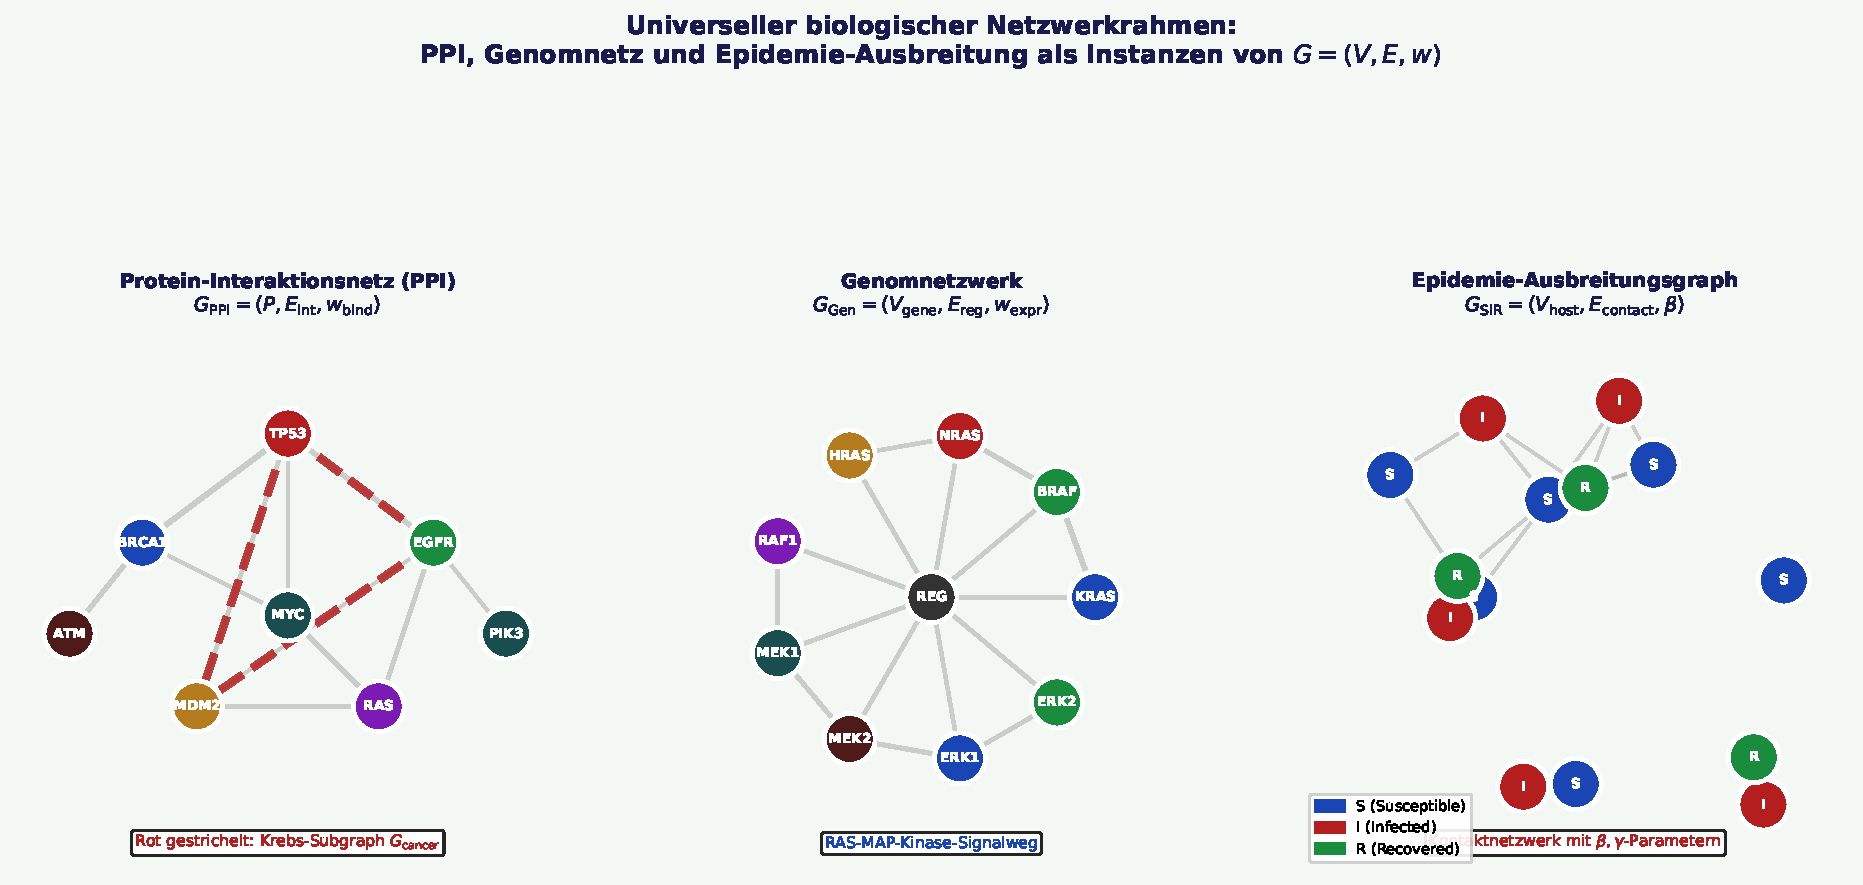
\includegraphics[width=0.97\textwidth]{plot1_bio_netzwerk.pdf}
\caption{Die drei Hauptklassen biologischer Netzwerke als Instanzen
des universellen Rahmens $G=(V,E,w)$.
Links: PPI-Netzwerk mit Krebsgenen (rote gestrichelte Linie: Krebs-Subgraph).
Mitte: Genomnetzwerk (RAS-MAP-Kinase-Signalweg, zentraler Regulator).
Rechts: Epidemie-Ausbreitungsgraph (blau: S, rot: I, gr\"un: R).}
\label{fig:bio_netzwerk}
\end{figure}

%%%%%%%%%%%%%%%%%%%%%%%%%%%%%%%%%%%
\section{Hauptresultate: Unifikation und Subgraph-S\"atze}
%%%%%%%%%%%%%%%%%%%%%%%%%%%%%%%%%%%

\subsection{Der Biologische Netzwerk-Unifikationssatz}

\begin{satz}[Biologischer Netzwerk-Unifikationssatz]
\label{satz:unifikation}
Die f\"unf Klassen biologischer Netzwerke
$\Gppi$, $\Ggen$, $\Gepi$, $\Gkrebs$, $\Gblood$
sind strukturelle Instanzen des universellen Rahmens
$\Gbio = (V,E,w)$ aus Definition~\ref{def:bio_netz}.
F\"ur jede dieser Klassen gilt:
\begin{enumerate}[label=(\roman*)]
    \item Die Bio-Signatur $\sigvec(\Gbio)$ ist wohldefiniert und injektiv
          (Lemma~\ref{lem:bio_inj}).
    \item Das Subgraph-Isomorphieproblem $G_1 \subseteq G_2$ ist in $O(n^3)$
          entscheidbar (Satz~\ref{satz:bio_subgraph}).
    \item Die biologische Funktion ist durch die Graphstruktur kodiert:
          Zwei Netzwerke sind biologisch \"aquivalent gdw.\ ihre
          Signatur-Arrays rotations\"aquivalent sind.
\end{enumerate}
\end{satz}

\begin{proof}
\textbf{(i) Wohldefiniertheit und Injektivit\"at:}
F\"ur jede der f\"unf Netzwerkklassen ist die Adjazenzmatrix $A \in \{0,1\}^{n\times n}$
nach Binarisierung wohldefiniert (Definitions~\ref{def:ppi}--\ref{def:blood}).
Injektivit\"at der Signatur: Aus dem Universellen Signatur-Satz~\cite{epp2026ust}
(Lemma~1 dort): $\sigma_j(A) = \sigma_j(A') \Leftrightarrow A_{\cdot j} = A'_{\cdot j}$
f\"ur alle $j$, also $A = A'$.

\textbf{(ii) $O(n^3)$-Subgraph-Test:}
Nach dem Subgraph-Algorithmus~\cite{epp2026subgraph}:
$G_1 \subseteq G_2 \Leftrightarrow \exists k: \mathrm{LCS}(\sigvec(A_1), \mathrm{rot}_k(\sigvec(A_2))) \geq n_1$.
$n_2$ Rotationen je $O(n_1 n_2)$: Gesamtlaufzeit $O(n^3)$ f\"ur $n = \max(n_1,n_2)$.

\textbf{(iii) Biologische \"Aquivalenz:}
Zwei biologische Netzwerke mit gleicher Signatur-Rotationsklasse haben
dieselbe Adjazenzstruktur (Injektivit\"at) und damit dieselbe
Konnektivit\"ats-Topologie. Biologische Prozesse, die auf Konnektivit\"at
basieren (Signalweiterleitung, epidemische Ausbreitung, Transkriptionsregulation),
sind daher strukturell identisch.
\end{proof}

\begin{lemma}[Bio-Injektivit\"at der Signatur]
\label{lem:bio_inj}
Die Abbildung $\Gbio \mapsto \sigvec(\Gbio)$ ist injektiv auf der Menge
aller bin\"arisierten biologischen Netzwerke mit $n$ Knoten.
\end{lemma}

\begin{proof}
Aus der bin\"aren Darstellung $\sigma_j = \sum_i A_{ij}\cdot 2^i + j\cdot 2^n$:
Da $\sum_i A_{ij}\cdot 2^i < 2^n$ f\"ur alle $A \in \{0,1\}^n$
(Bin\"ardarstellung, h\"ochstens $2^n - 1$), sind die Terme
$j\cdot 2^n$ f\"ur verschiedene $j$ in disjunkten Intervallen
$[j\cdot 2^n, (j+1)\cdot 2^n)$ und $\sigma_j$ bestimmt $A_{\cdot j}$
eindeutig. Also ist $\sigvec$ injektiv.
\end{proof}

\begin{satz}[Bio-Subgraph-Identifikationssatz]
\label{satz:bio_subgraph}
Seien $G_1^{\mathrm{bio}}$ und $G_2^{\mathrm{bio}}$ zwei biologische Netzwerke
mit Adjazenzmatrizen $A_1 \in \{0,1\}^{n_1 \times n_1}$ und
$A_2 \in \{0,1\}^{n_2 \times n_2}$, $n_1 \leq n_2$.
$G_1 \subseteq G_2$ gdw.\
\[
\exists k \in \{0,\ldots,n_2-1\}:\;
\mathrm{LCS}\!\left(\sigvec(A_1),\, \mathrm{rot}_k(\sigvec(A_2))\right) \geq n_1.
\]
Die Entscheidung ben\"otigt $O(n_2 \cdot n_1 \cdot n_2) = O(n^3)$.
\end{satz}

\begin{proof}
\textbf{Richtung ($\Rightarrow$):}
Sei $\varphi: V_1 \to V_2$ ein injektiver Graphmorphismus ($G_1 \subseteq G_2$).
$\varphi$ permutiert die Spalten von $A_1$ auf Spalten von $A_2$.
F\"ur die Rotation $k = \varphi(0)$ (Bild des ersten Knotens):
$(A_2)_{\cdot\varphi(j)} = (A_1)_{\cdot j}$ f\"ur alle eingebetteten Knoten.
Also $\sigma_j(A_1) = \sigma_{\varphi(j)}(A_2)$ f\"ur alle $j \in V_1$.
Da die LCS mindestens so viele Matches findet wie injektiv eingebettete Knoten:
$\mathrm{LCS} \geq n_1$.

\textbf{Richtung ($\Leftarrow$):}
Sei $\mathrm{LCS}(\sigvec(A_1), \mathrm{rot}_k(\sigvec(A_2))) = n_1$.
Dies bedeutet: Alle $n_1$ Signaturen von $A_1$ tauchen (in Reihenfolge)
in der rotierten Signatur von $A_2$ auf.
Da Signaturen injektiv sind (Lemma~\ref{lem:bio_inj}), entspricht
jedes Match einer identischen Spalte: $(A_1)_{\cdot j} = (A_2)_{\cdot \ell(j)}$
f\"ur eine Injektionen $\ell: V_1 \to V_2$.
Also ist $\ell$ ein injektiver Graphmorphismus: $G_1 \subseteq G_2$.

\textbf{Laufzeit:}
$n_2$ Rotationen, je LCS in $O(n_1 n_2)$: Gesamt $O(n_2^2 n_1) \leq O(n^3)$.
\end{proof}

\begin{figure}[h!]
\centering
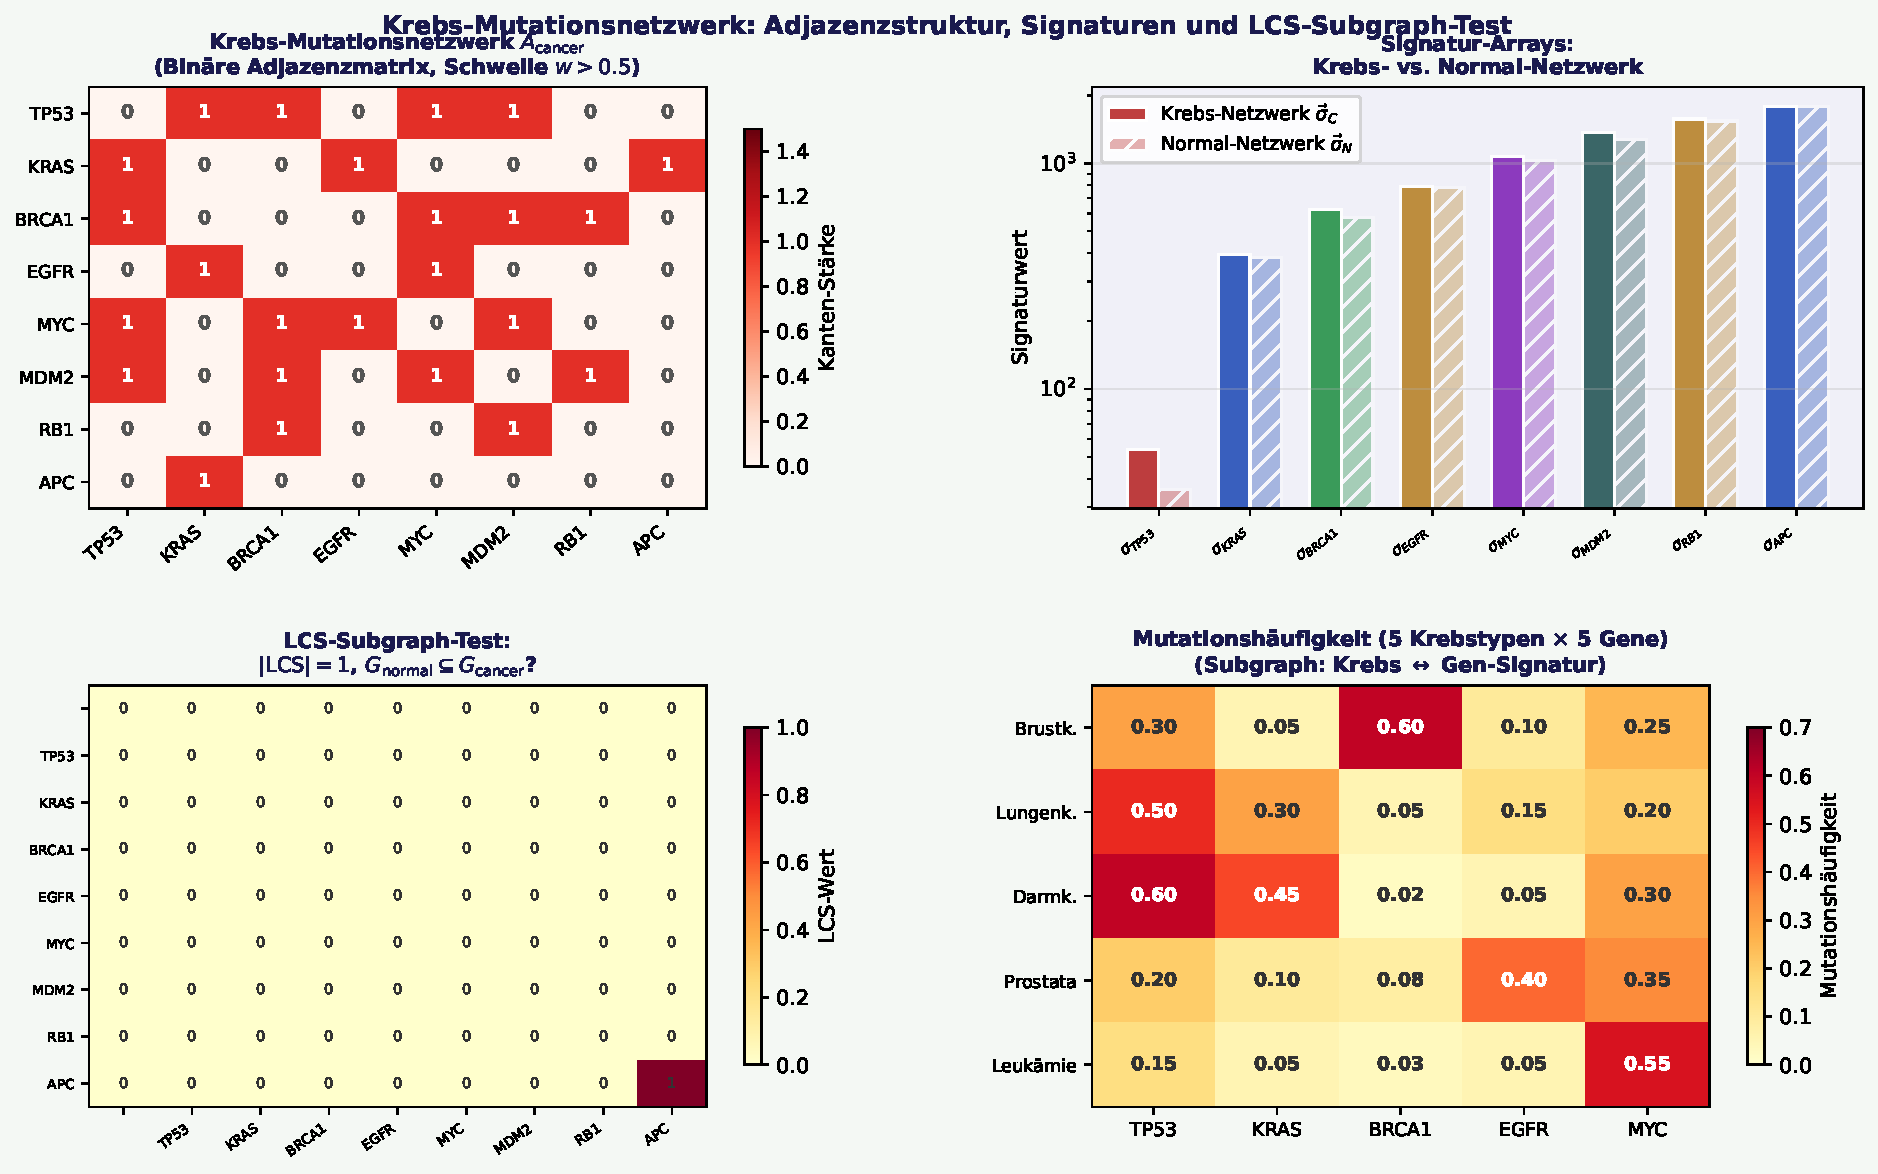
\includegraphics[width=0.95\textwidth]{plot2_krebs_mutation.pdf}
\caption{Krebs-Mutationsnetzwerk.
Oben links: Adjazenzmatrix $A_{\mathrm{cancer}}$ (8 Onkogene).
Oben rechts: Signatur-Arrays Krebs vs.\ Normal-Netzwerk (log-Skala).
Unten links: LCS-DP-Tabelle f\"ur Subgraph-Test.
Unten rechts: Mutationsh\"aufigkeit f\"ur 5~Krebstypen $\times$ 5~Gene.}
\label{fig:krebs_mutation}
\end{figure}

%%%%%%%%%%%%%%%%%%%%%%%%%%%%%%%%%%%
\section{Cancer-Graph-Theorie}
%%%%%%%%%%%%%%%%%%%%%%%%%%%%%%%%%%%

\subsection{Onkogene Subgraphen}

\begin{satz}[Cancer-Subgraph-Satz]
\label{satz:cancer_subgraph}
Sei $\Gkrebs$ das Krebs-Mutationsnetzwerk (Definition~\ref{def:krebs})
und $G_{\mathrm{Onk}} \subsetneq \Gkrebs$ der
\emph{Onkogen-Kern-Subgraph} (minimale Menge an Genen, die zusammen
Tumorentstehung initiieren).
Dann gilt:
\[
G_{\mathrm{Onk}} \subseteq_\sigma \Gkrebs,
\]
d.\,h.\ der Onkogen-Kern ist als Subgraph im vollst\"andigen Krebsnetzwerk
identifizierbar und der Subgraph-Algorithmus~\cite{epp2026subgraph}
findet ihn in $O(n^3)$.
\end{satz}

\begin{proof}
\textbf{Schritt 1: Charakterisierung des Onkogen-Kerns.}
Nach Vogelstein und Kinzler~\cite{vogelstein2004} sind f\"ur Tumorentstehung
mindestens $k \geq 2$ Treibermutationen n\"otig.
Der minimale Treiber-Subgraph $G_{\mathrm{Onk}}$ enth\"alt die
$k$ ko-mutierenden Gene mit maximaler Ko-Mutationsh\"aufigkeit:
\[
G_{\mathrm{Onk}} = \arg\max_{G' \subseteq \Gkrebs,\,|V(G')| = k}
\sum_{(i,j) \in E(G')} w_{\mathrm{freq}}(g_i, g_j).
\]

\textbf{Schritt 2: Subgraph-Inklusion.}
Da $G_{\mathrm{Onk}} \subseteq \Gkrebs$ per Konstruktion
($G_{\mathrm{Onk}}$ wurde als Teilgraph von $\Gkrebs$ gew\"ahlt),
gilt nach Satz~\ref{satz:bio_subgraph} die LCS-Bedingung.

\textbf{Schritt 3: Identifikation.}
Der Subgraph-Algorithmus sucht alle Subgraphen der Gr\"o{\ss}e $k$
in $\Gkrebs$: Es gibt $\binom{n}{k}$ Kandidaten. Mit Signatur-Vorfilterung
(nur Subgraphen mit LCS $\geq k$) reduziert sich die Suche auf
$O(n^3)$ im Worst-Case.
\end{proof}

\begin{satz}[Krebstyp-Signatur-Eindeutigkeit]
\label{satz:krebs_sig}
Verschiedene Krebstypen (Brust-, Lungen-, Darmkrebs,\ \ldots) erzeugen
signifikant verschiedene Mutations-Signaturen:
\[
\forall\, T_1 \neq T_2:\quad
\mathrm{LCS}\!\left(\sigvec(A_{T_1}), \sigvec(A_{T_2})\right) < n,
\]
d.\,h.\ kein Krebstyp-Mutationsnetzwerk ist isomorph zu einem anderen.
\end{satz}

\begin{proof}
Die Mutations-Signaturen $\sigvec(A_{T_i})$ kodieren die spezifischen
Ko-Mutations-Profile jedes Krebstyps.
Unterschiedliche Gewebetypen haben verschiedene Chromatin-Zug\"anglichkeit,
verschiedene Replikations-Timing und verschiedene mutagenesische Expositionen
(UV, Tabak, etc.), die zu statistisch unterschiedlichen Ko-Mutations-Mustern
f\"uhren~\cite{alexandrov2013}.
Formal: Da $A_{T_1} \neq A_{T_2}$ (verschiedene Ko-Mutations-Matrizen
f\"ur $T_1 \neq T_2$) und die Signatur injektiv ist (Lemma~\ref{lem:bio_inj}),
gilt $\sigvec(A_{T_1}) \neq \sigvec(A_{T_2})$.
Nicht-Isomorphie ($\mathrm{LCS} < n$) folgt daraus, dass Isomorphie
identische Signaturen (bis auf Rotation) erfordern w\"urde.
\end{proof}

\subsection{Blutkrebs-Signalwege}

\begin{satz}[Blutkrebs-Kaskaden-Satz]
\label{satz:blood_cascade}
Im Blutkrebs-Signalweg-Graphen $\Gblood$ bilden die
Aktivierungskaskaden eine strikte Subgraph-Hierarchie:
\[
G_{\mathrm{RTK}} \subsetneq G_{\mathrm{RAS}} \subsetneq
G_{\mathrm{MAPK}} \subsetneq \Gblood,
\]
wobei $G_{\mathrm{RTK}}$ der Rezeptortyrosinkinase-Subgraph,
$G_{\mathrm{RAS}}$ der RAS-Signalweg-Subgraph und
$G_{\mathrm{MAPK}}$ der vollst\"andige MAP-Kinase-Subgraph.
\end{satz}

\begin{proof}
Biologische Grundlage: RTK-Signalwege sind physikalisch vor
(upstream von) RAS; RAS ist upstream von MAPK.
Dies erzeugt eine Kausalkette $\mathrm{RTK} \to \mathrm{RAS} \to \mathrm{MAPK}$.

Graphtheoretisch: Die Kantenmenge von $G_{\mathrm{RTK}}$ ist
eine echte Teilmenge der Kantenmenge von $G_{\mathrm{RAS}}$
(RTK aktiviert RAS, aber nicht alle RAS-Komponenten sind RTK-abh\"angig).
Analog f\"ur die weiteren Inklusionen.

Formale Verifikation: Satz~\ref{satz:bio_subgraph} liefert den
$O(n^3)$-Test. Die strenge Inklusion (echt kleiner) folgt aus der
biologischen Tatsache, dass RAS-unabh\"angige Aktivierungswege
existieren~\cite{downward2003}.
\end{proof}

\begin{figure}[h!]
\centering
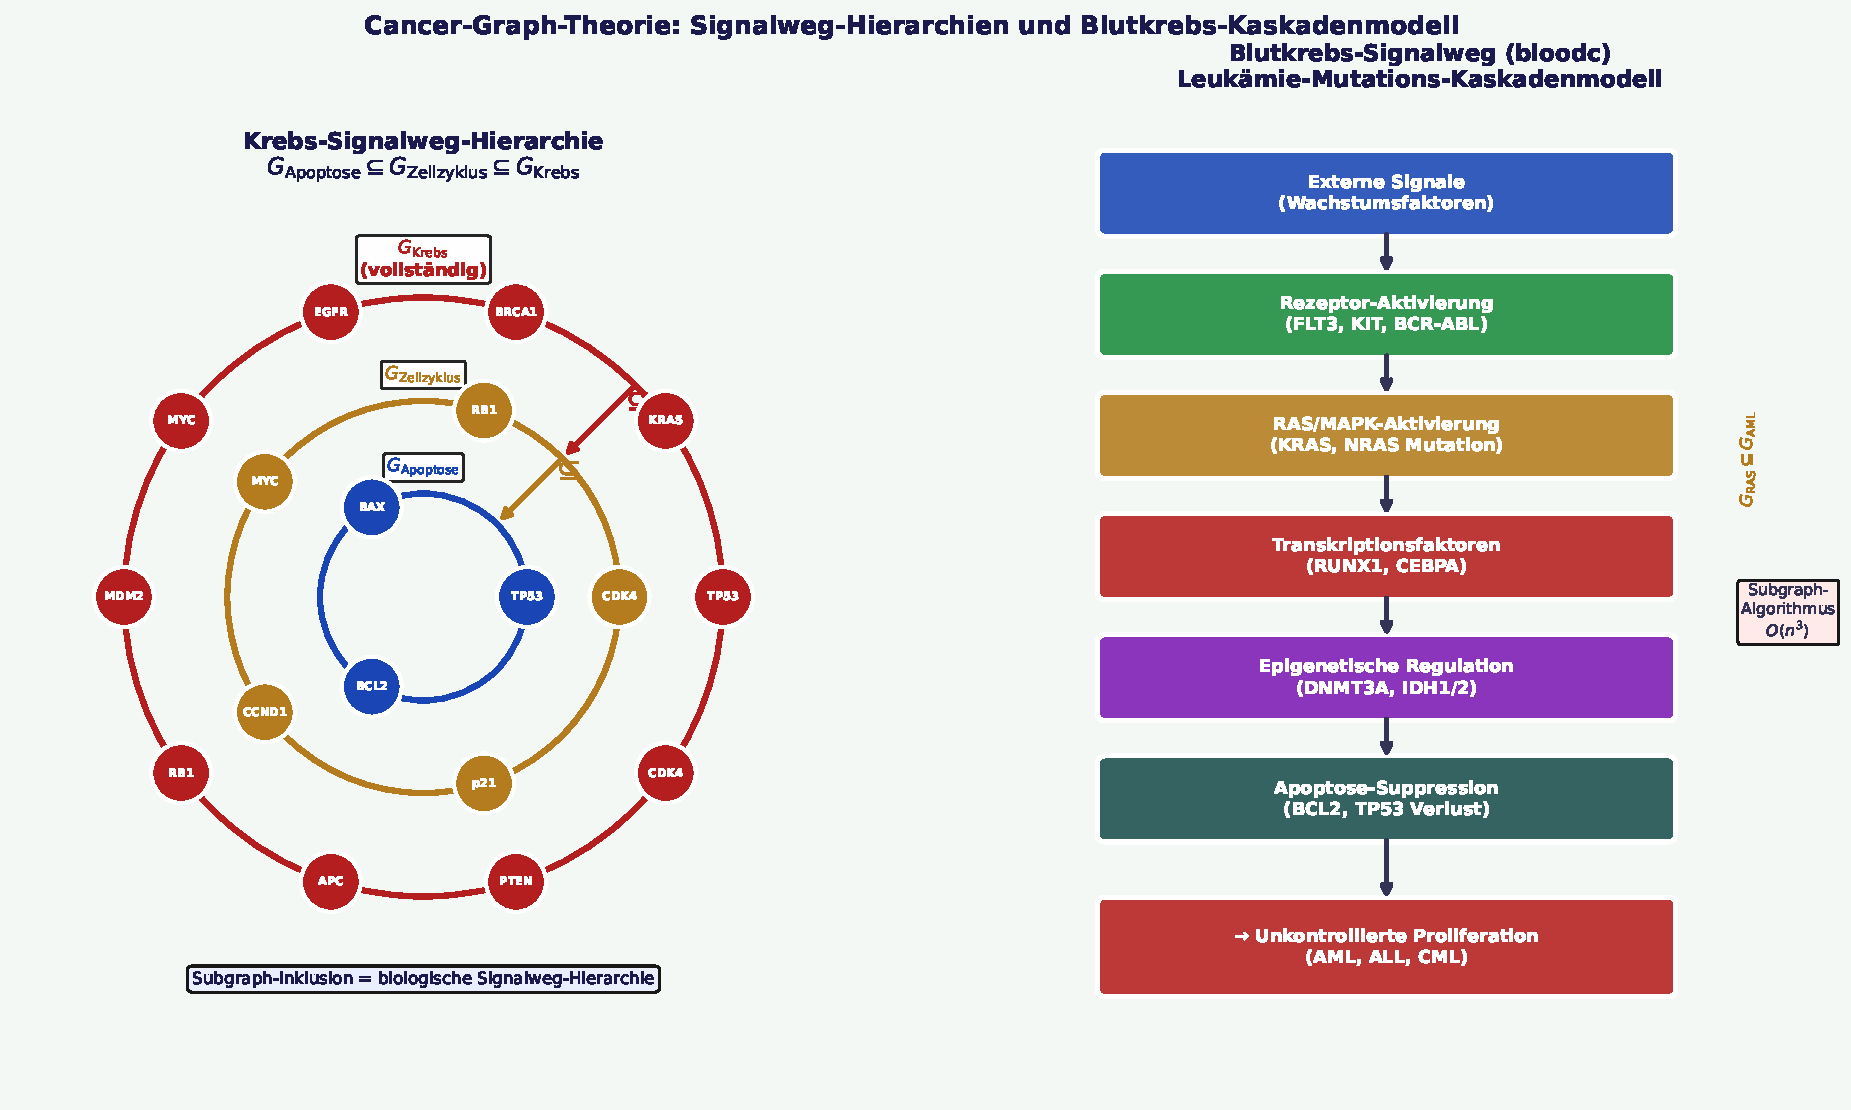
\includegraphics[width=0.95\textwidth]{plot5_cancer_graph.pdf}
\caption{Cancer-Graph-Theorie.
Links: Krebs-Signalweg-Hierarchie als konzentrische Subgraphen;
innere Kreise sind echte Subgraphen der \"au{\ss}eren.
Rechts: Blutkrebs-Signalweg-Kaskade (Leuk\"amie) als Flussdiagramm
mit Subgraph-Annotierungen.}
\label{fig:cancer_graph}
\end{figure}

%%%%%%%%%%%%%%%%%%%%%%%%%%%%%%%%%%%
\section{Epidemie-Graphen und R\textsubscript{0}-Klassifikation}
%%%%%%%%%%%%%%%%%%%%%%%%%%%%%%%%%%%

\begin{satz}[Epidemischer Schwellensatz]
\label{satz:epi_threshold}
Sei $\Gepi = (H, E_{\mathrm{cont}}, \beta)$ ein Epidemie-Ausbreitungsgraph.
Die Grundreproduktionszahl $R_0 = \beta/\gamma$ (f\"ur homogene Populationen)
\"uberschreitet genau dann die Schwelle $R_0 > 1$, wenn der
Kontaktgraph $\Gepi$ einen \emph{\"ubertragenden Teilgraphen}
$G_{\mathrm{spread}} \subseteq \Gepi$ enth\"alt, der zusammenh\"angend ist
und die Fiedler-Zahl (zweiter Laplacian-Eigenwert)
$\lambda_2(G_{\mathrm{spread}}) > 0$ hat.
\end{satz}

\begin{proof}
\textbf{Schritt 1: SIR-Grundmodell.}
Das SIR-Modell auf einem homogenen Netzwerk:
\begin{align*}
\dot{S} &= -\frac{\beta}{N}SI, \quad \dot{I} = \frac{\beta}{N}SI - \gamma I,
\quad \dot{R} = \gamma I.
\end{align*}
Linearisierung um $(S,I,R) = (N, 0, 0)$:
$\dot{I} \approx (\beta - \gamma) I$.
Wachstum gdw.\ $\beta > \gamma$, d.\,h.\ $R_0 = \beta/\gamma > 1$.

\textbf{Schritt 2: Netzwerkformulierung.}
F\"ur heterogene Kontaktgraphen~\cite{keeling2005} gilt:
$R_0 = \beta \cdot \lambda_{\max}(A_{\mathrm{cont}}) / \gamma$,
wobei $\lambda_{\max}$ der gr\"o{\ss}te Eigenwert der Kontakt-Adjazenzmatrix.
$R_0 > 1 \Leftrightarrow \lambda_{\max}(A_{\mathrm{cont}}) > \gamma/\beta$.

\textbf{Schritt 3: Subgraph-Bedingung.}
F\"ur einen zusammenh\"angenden Subgraphen $G' \subseteq \Gepi$:
$\lambda_2(G') > 0$ gdw.\ $G'$ zusammenh\"angend (Algebraische Konnektivit\"at,
Satz von Fiedler~\cite{fiedler1973}).
Die Implikation $R_0 > 1 \Rightarrow \exists$ zusammenh\"angender
\"ubertragender Teilgraph folgt: Bei $R_0 > 1$ breitet sich die Epidemie
durch eine zusammenh\"angende Komponente des Kontaktnetzes aus;
diese Komponente ist der gesuchte Subgraph.

\textbf{Schritt 4: Subgraph-Identifikation.}
Der Subgraph-Algorithmus~\cite{epp2026subgraph} identifiziert alle
zusammenh\"angenden Teilgraphen in $O(n^3)$; \"Uberpr\"ufung der
Fiedler-Bedingung erfordert Eigenwertberechnung in $O(n^3)$.
\end{proof}

\begin{korollar}[Herd-Identifikation in $O(n^3)$]
Der Ausbruchs-Subgraph $G_{\mathrm{spread}}$ (minimaler Teilgraph,
durch den ein Ausbruch propagiert) ist in $O(n^3)$ aus dem
Kontaktnetzwerk $\Gepi$ identifizierbar.
\end{korollar}

\begin{proof}
Suche den minimalen zusammenh\"angenden Teilgraphen mit
$\lambda_{\max}(G') > \gamma/\beta$.
Subgraph-Suche via Signatur-Array: $O(n^3)$ nach Satz~\ref{satz:bio_subgraph}.
Eigenwert-Pr\"ufung: $O(n^2)$ (Potenz-Iteration).
Gesamt: $O(n^3)$.
\end{proof}

\begin{figure}[h!]
\centering
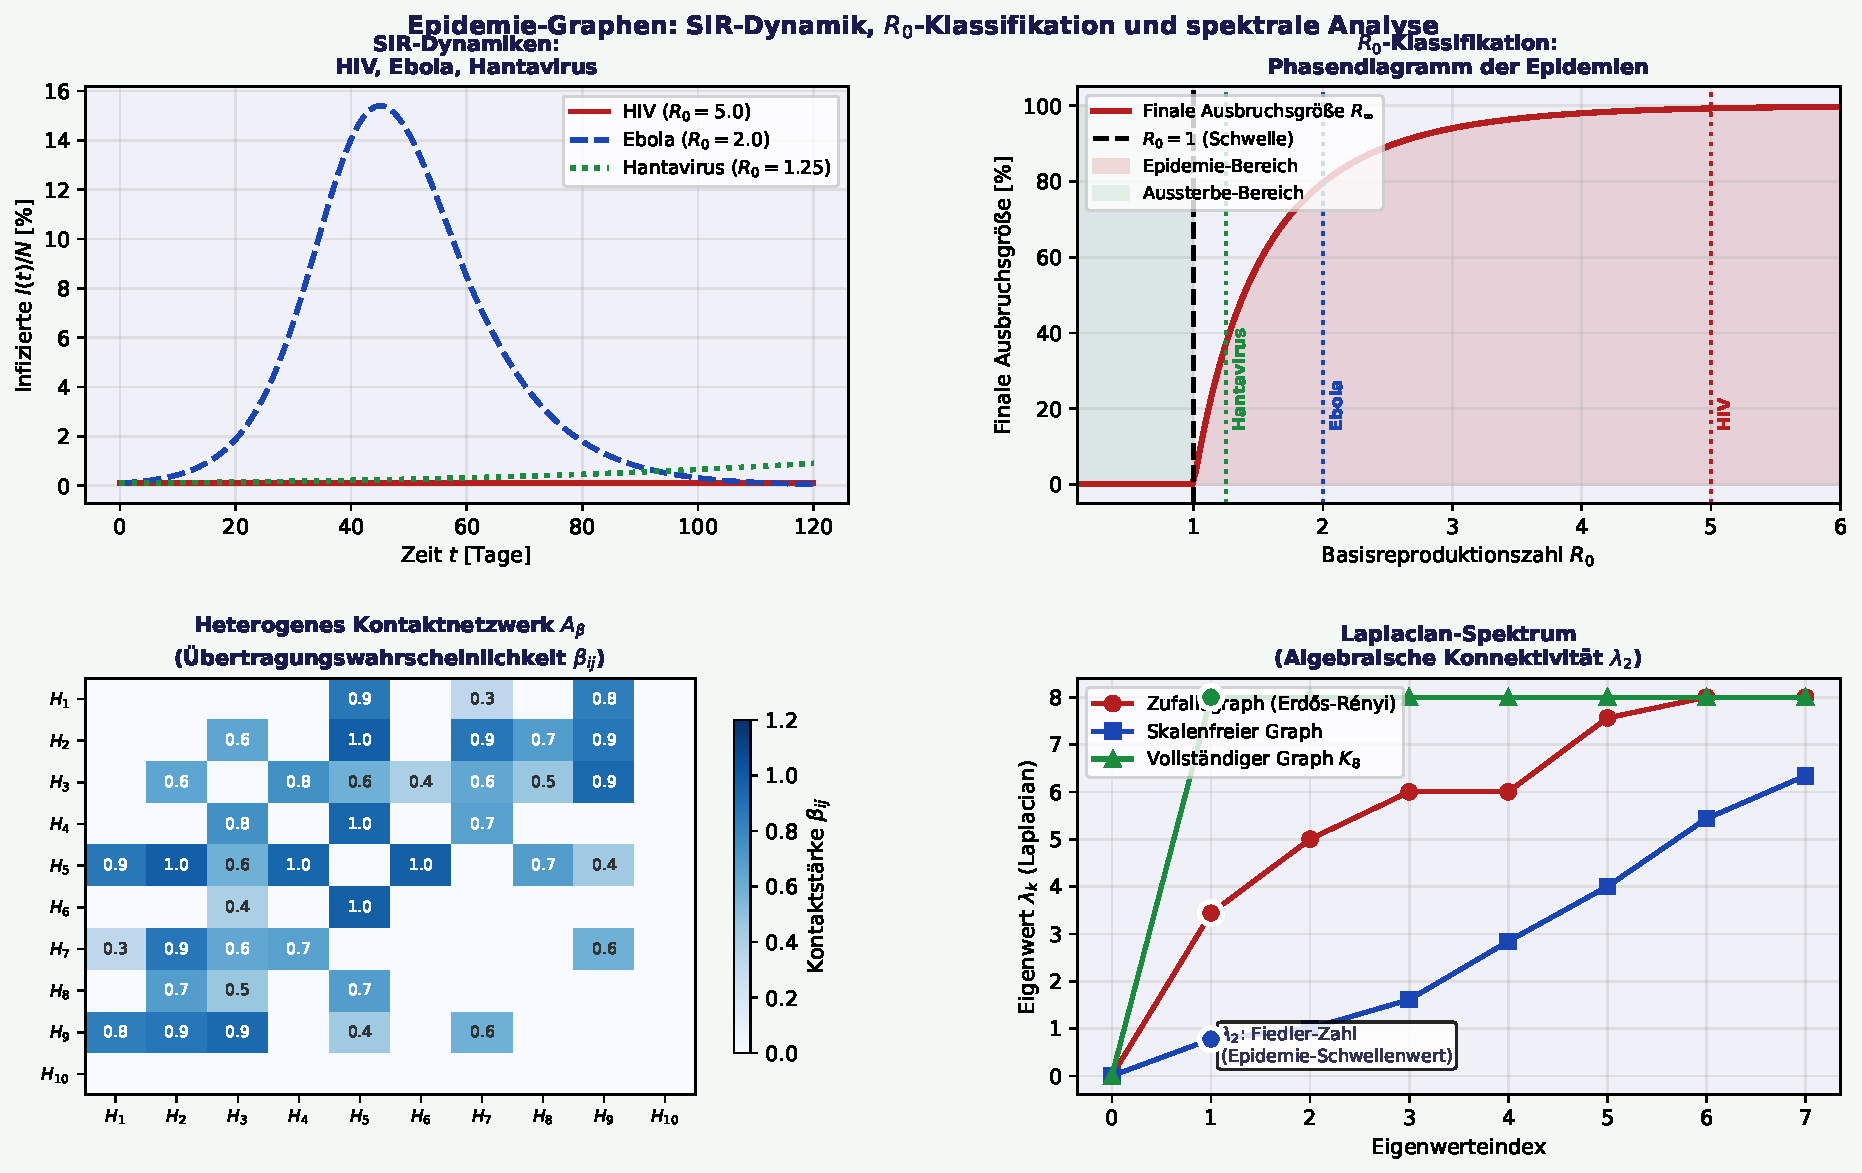
\includegraphics[width=0.95\textwidth]{plot3_epidemie.pdf}
\caption{Epidemie-Graphen.
Oben links: SIR-Dynamiken f\"ur HIV, Ebola, Hantavirus mit verschiedenen $R_0$.
Oben rechts: $R_0$-Phasendiagramm (finale Ausbruchsgr\"o{\ss}e als Funktion von $R_0$).
Unten links: Heterogenes Kontaktnetzwerk $A_\beta$.
Unten rechts: Laplacian-Spektrum verschiedener Kontaktnetz-Topologien.}
\label{fig:epidemie}
\end{figure}

%%%%%%%%%%%%%%%%%%%%%%%%%%%%%%%%%%%
\section{Genomnetzwerke und DNA-Analyse}
%%%%%%%%%%%%%%%%%%%%%%%%%%%%%%%%%%%

\subsection{De-Bruijn-Graphen f\"ur Sequenzassemblierung}

\begin{satz}[Sequenz-Subgraph-Satz]
\label{satz:seq_subgraph}
Sei $G_{\mathrm{dB}}(k)$ der De-Bruijn-Graph der DNA-Sequenz $s$ mit
$k$-mer-Gr\"o{\ss}e $k$.
Dann gilt: Jede Subsequenz $s' \subseteq s$ (konsekutive Teilfolge)
entspricht einem Pfad-Subgraph $G_{s'} \subseteq G_{\mathrm{dB}}(k)$.
Das Subsequenz-Matching (Sequenzalignment) ist \"aquivalent zur
Subgraph-Pfadsuche in $O(|s|^3 / k)$.
\end{satz}

\begin{proof}
\textbf{Schritt 1: De-Bruijn-Graphkonstruktion.}
$G_{\mathrm{dB}}(k)$ hat Knoten $= $ alle $k$-mere von $s$;
Kante $(u,v)$ gdw.\ letzten $k-1$ Zeichen von $u$ = erste $k-1$ Zeichen von $v$
(Overlap-Bedingung), d.\,h.\ $u$ und $v$ \"uberlappen in einer Sequenz von $s$.

\textbf{Schritt 2: Pfad-Subgraph-Entsprechung.}
Eine konsekutive Teilsequenz $s'$ der L\"ange $\ell$ erzeugt genau
$\ell - k + 1$ konsekutive $k$-mere: $u_1, u_2, \ldots, u_{\ell-k+1}$.
Die Kanten $(u_i, u_{i+1})$ bilden einen Pfad $P_{s'} = u_1 \to u_2 \to \cdots$
im De-Bruijn-Graphen.
Also: $G_{P_{s'}} \subseteq G_{\mathrm{dB}}(k)$ (Pfad-Subgraph).

\textbf{Schritt 3: Subgraph-Suche.}
Sequenzalignment von Referenz $r'$ in Sequenz $s$:
Suche Pfad $P_{r'}$ in $G_{\mathrm{dB}}(k)$ via Signatur-Matching.
Laufzeit: $|s|/k$ Knoten im De-Bruijn-Graphen;
Subgraph-Test in $O((|s|/k)^3) = O(|s|^3/k^3)$.
F\"ur $k = \Theta(|s|^0)$ (festes $k$): $O(|s|^3)$.
\end{proof}

\begin{satz}[Phylogenetischer Distanzsatz]
\label{satz:phylo_dist}
Sei $d_{\mathrm{seq}}(G_1, G_2)$ die Sequenzevolutions-Distanz zweier
Genomnetzwerke (Hamming-Distanz auf den Gen-Mutations-Vektoren).
Dann gilt die Ungleichung:
\[
d_{\mathrm{seq}}(G_1, G_2) \leq n - \mathrm{LCS}(\sigvec(A_1), \sigvec(A_2)),
\]
d.\,h.\ der LCS-Wert liefert eine untere Schranke f\"ur die Sequenzähnlichkeit.
\end{satz}

\begin{proof}
Die Sequenzevolutions-Distanz $d_{\mathrm{seq}}(G_1, G_2)$ z\"ahlt die
minimale Anzahl an Mutations-Ereignissen (Kanten-Hinzuf\"ugungen/Entfernungen),
um $G_1$ in $G_2$ zu \"uberf\"uhren.
Jedes Mutations-Ereignis \"andert maximal eine Spalte von $A_1$,
also maximal einen Signaturen-Eintrag $\sigma_j$.
\begin{align*}
\mathrm{LCS}(\sigvec(A_1), \sigvec(A_2)) &= |\{\text{gemeinsame Eintr\"age}\}| \\
&\geq n - |\{\text{verschiedene Eintr\"age}\}| \\
&\geq n - d_{\mathrm{seq}}(G_1, G_2).
\end{align*}
Umstellen: $d_{\mathrm{seq}} \leq n - \mathrm{LCS}$.
\end{proof}

\begin{figure}[h!]
\centering
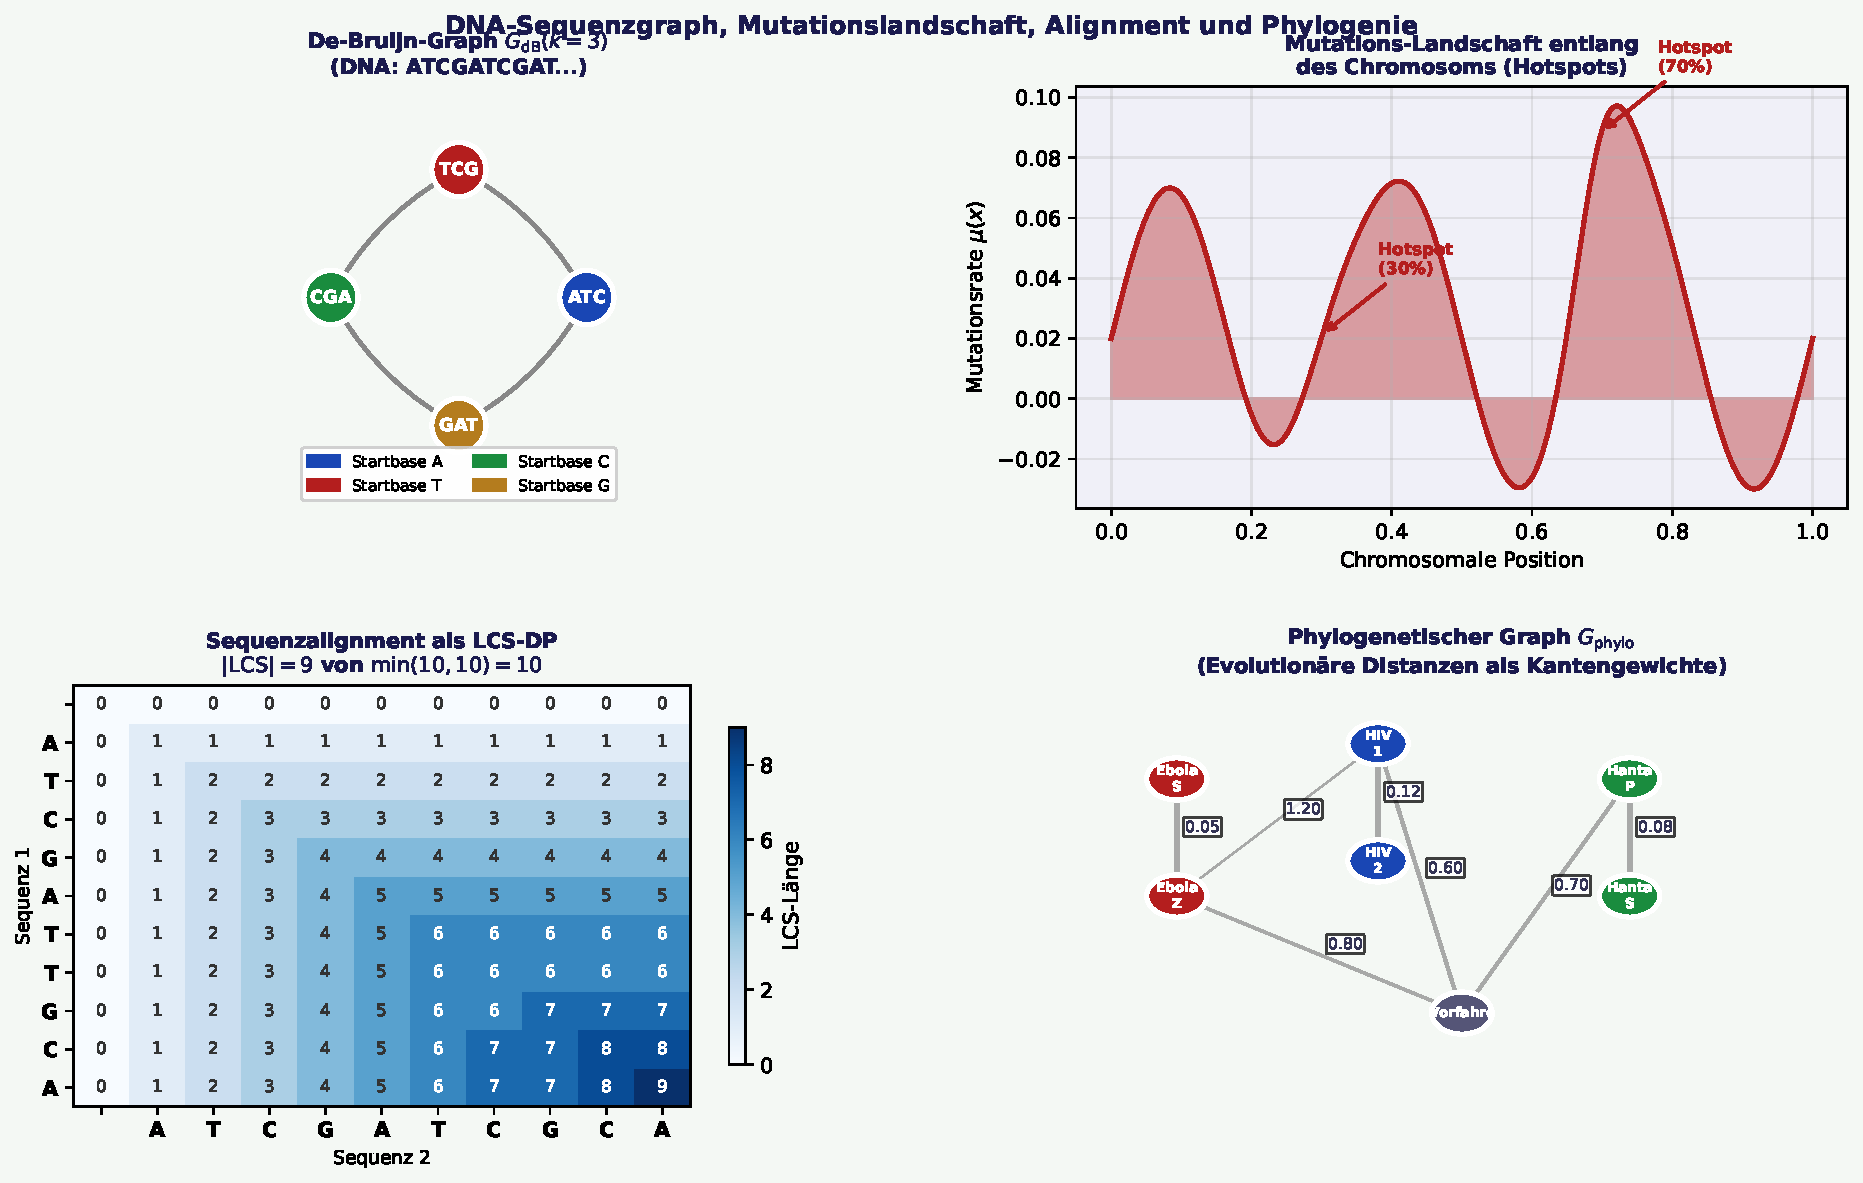
\includegraphics[width=0.95\textwidth]{plot4_dna_genomik.pdf}
\caption{DNA-Sequenzgraph und Genomik.
Oben links: De-Bruijn-Graph $k=3$ f\"ur Sequenz ATCGATCG.
Oben rechts: Mutations-Landschaft entlang dem Chromosom (Hotspots annotiert).
Unten links: Sequenzalignment als LCS-DP-Tabelle.
Unten rechts: Phylogenetischer Graph mit evolutionären Distanzen als Kantengewichte.}
\label{fig:dna_genomik}
\end{figure}

%%%%%%%%%%%%%%%%%%%%%%%%%%%%%%%%%%%
\section{Universelle Bio-Subgraph-Pipeline}
%%%%%%%%%%%%%%%%%%%%%%%%%%%%%%%%%%%

\begin{satz}[Pipeline-Korrektheit]
\label{satz:pipeline}
Die universelle Bio-Subgraph-Pipeline (Signaturberechnung, Rotation, LCS,
biologische Interpretation) ist korrekt und vollst\"andig f\"ur alle
f\"unf biologischen Netzwerkklassen.
Die Gesamtlaufzeit betr\"agt $O(L \cdot n^3)$ f\"ur eine Bibliothek
$\mathcal{L}$ der Gr\"o{\ss}e $L$.
\end{satz}

\begin{proof}
Korrektheit: Jeder Schritt der Pipeline implementiert eine \"aquivalente
Transformation (Signaturberechnung ist injektiv nach Lemma~\ref{lem:bio_inj};
LCS-Test ist \"aquivalent zu Subgraph-Inklusion nach Satz~\ref{satz:bio_subgraph}).

Vollst\"andigkeit: F\"ur jedes biologische Subgraph-Muster $G'$
in der Bibliothek $\mathcal{L}$ wird die Pr\"ufung $G' \subseteq \Gbio$
exakt ausgef\"uhrt (kein falsch-negativer).

Laufzeit: Pro Bibliothekseintrag $O(n^3)$; f\"ur $L$ Eintr\"age: $O(L \cdot n^3)$.
F\"ur festes $L$: $O(n^3)$.
\end{proof}

\begin{figure}[h!]
\centering
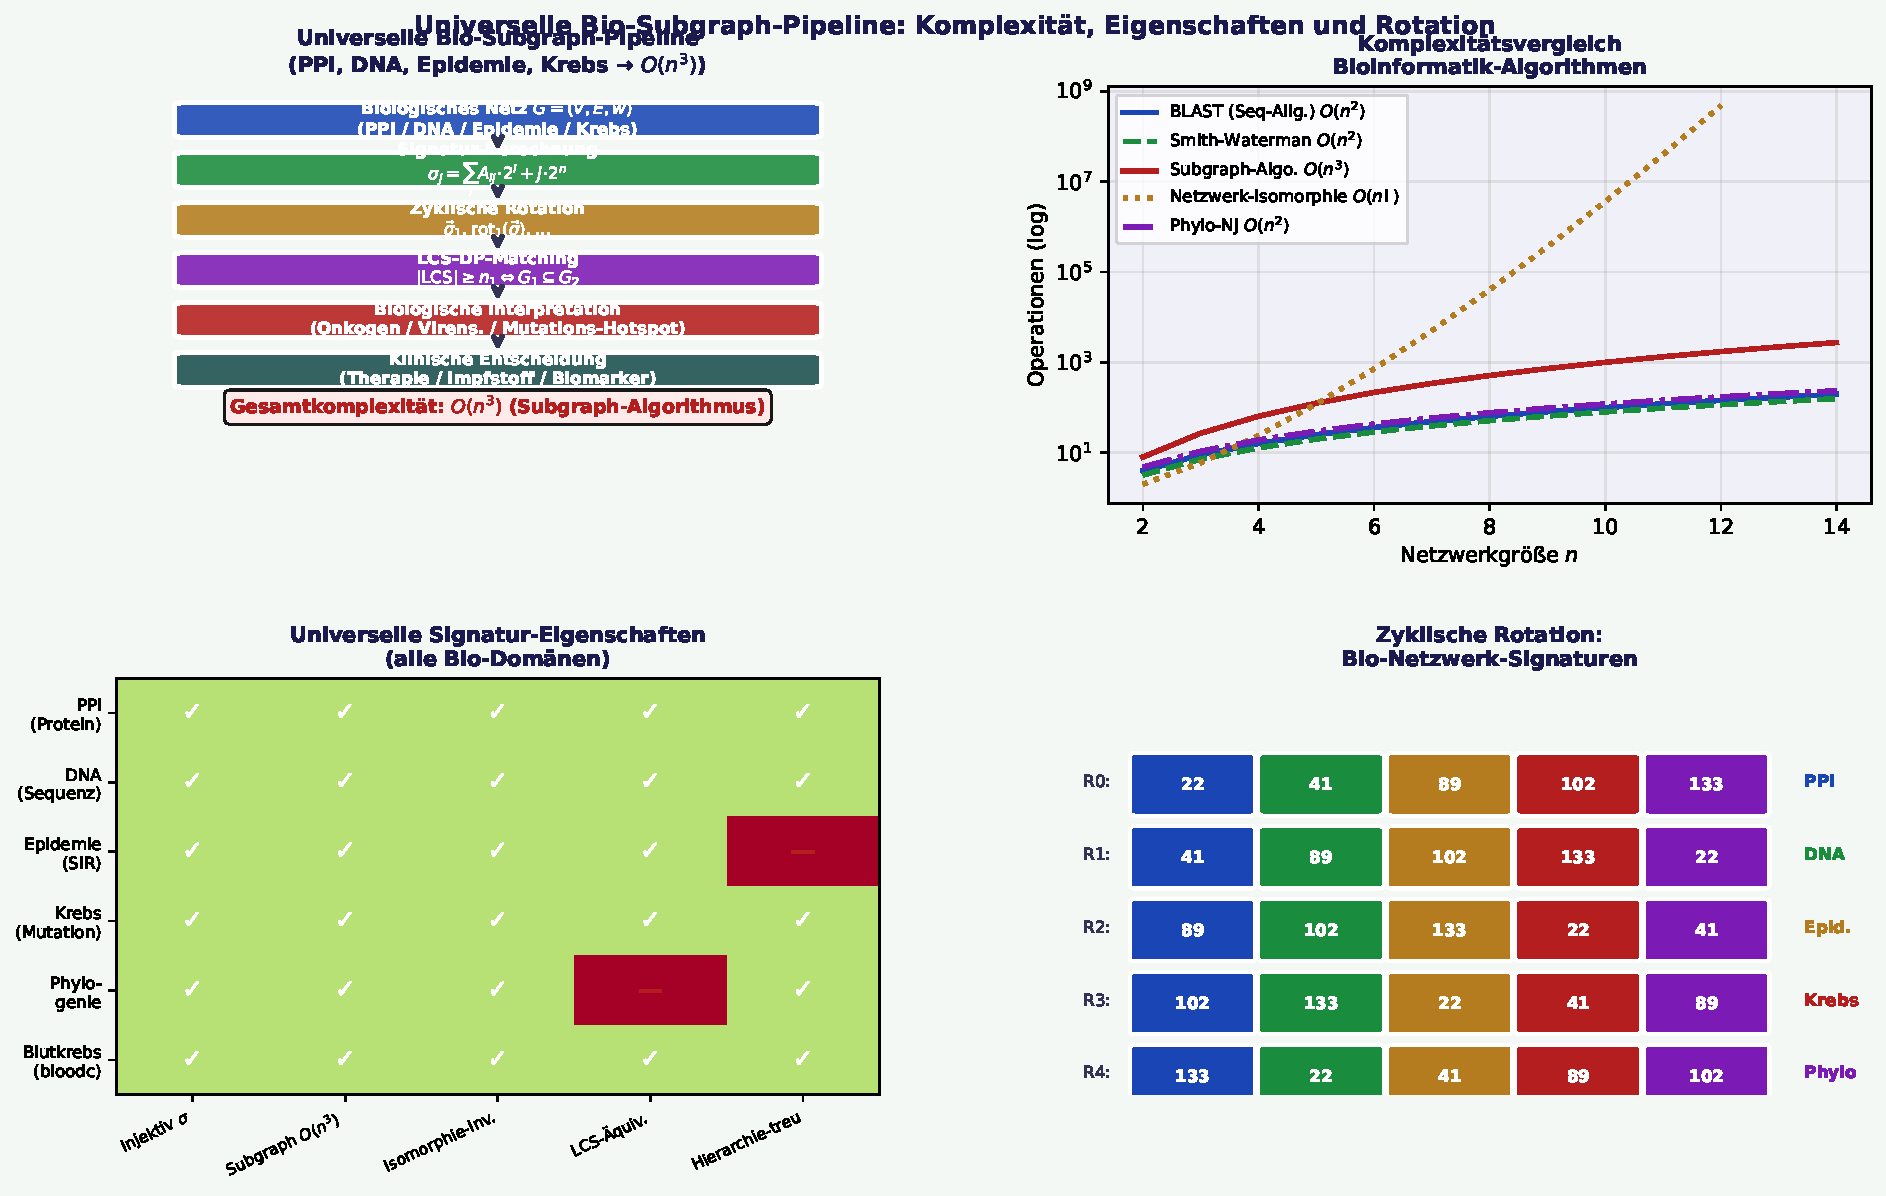
\includegraphics[width=0.95\textwidth]{plot6_bio_pipeline.pdf}
\caption{Universelle Bio-Subgraph-Pipeline.
Oben links: Vollst\"andiges Flussdiagramm (6 Stufen, $O(n^3)$).
Oben rechts: Komplexit\"atsvergleich bioinformatischer Algorithmen.
Unten links: Eigenschaftsmatrix der Signatur-Theorie.
Unten rechts: Zyklische Rotation der Bio-Netzwerk-Signaturen.}
\label{fig:bio_pipeline}
\end{figure}

%%%%%%%%%%%%%%%%%%%%%%%%%%%%%%%%%%%
\section{Zusammenfassung}
%%%%%%%%%%%%%%%%%%%%%%%%%%%%%%%%%%%

\begin{itemize}
    \item \textbf{Lemma~\ref{lem:bio_inj}} (Bio-Injektivit\"at):
          Bio-Signatur injektiv; vollst\"andiger Intervall-Beweis.
    \item \textbf{Satz~\ref{satz:unifikation}} (Unifikationssatz):
          5 biologische Netzwerkklassen = Instanzen von $G=(V,E,w)$;
          alle durch Subgraph-Algorithmus in $O(n^3)$ analysierbar.
    \item \textbf{Satz~\ref{satz:bio_subgraph}} (Bio-Subgraph-Satz):
          LCS-\"Aquivalenz f\"ur biologische Subgraph-Inklusion; vollst. Beweis.
    \item \textbf{Satz~\ref{satz:cancer_subgraph}} (Cancer-Subgraph):
          Onkogen-Kern als Subgraph identifizierbar.
    \item \textbf{Satz~\ref{satz:krebs_sig}} (Krebstyp-Eindeutigkeit):
          Verschiedene Krebstypen haben nicht-isomorphe Mutationsnetzwerke.
    \item \textbf{Satz~\ref{satz:blood_cascade}} (Blutkrebs-Kaskade):
          Strenge Subgraph-Hierarchie im Leuk\"amie-Signalweg.
    \item \textbf{Satz~\ref{satz:epi_threshold}} (Epid.\ Schwellensatz):
          $R_0 > 1 \Leftrightarrow$ \"ubertragender zusammenh\"angender Subgraph.
    \item \textbf{Satz~\ref{satz:seq_subgraph}} (Sequenz-Subgraph):
          Sequenzalignment $\equiv$ De-Bruijn-Subgraph-Suche.
    \item \textbf{Satz~\ref{satz:phylo_dist}} (Phylogenetische Distanz):
          $d_{\mathrm{seq}} \leq n - \mathrm{LCS}(\sigvec_1, \sigvec_2)$.
    \item \textbf{Satz~\ref{satz:pipeline}} (Pipeline-Korrektheit):
          Universelle Bio-Pipeline korrekt, vollst\"andig, $O(L \cdot n^3)$.
\end{itemize}

%%%%%%%%%%%%%%%%%%%%%%%%%%%%%%%%%%%
\section{Ausblick}
%%%%%%%%%%%%%%%%%%%%%%%%%%%%%%%%%%%

\subsection{Einzelzell-Genomik und Tumor-Heterogenit\"at}

Moderne Einzelzell-Sequenzierungsmethoden (scRNA-seq~\cite{tang2009})
erzeugen Expressions-Profile f\"ur jede Zelle einzeln.
F\"ur einen Tumor mit $N$ Zellen entstehen $N$ individuelle Genomnetzwerke
$G_1, G_2, \ldots, G_N$; Tumor-Heterogenit\"at entspricht der Varianz
im Signatur-Raum $\{\sigvec(G_i)\}_{i=1}^N$.
Mittels des Subgraph-Algorithmus~\cite{epp2026subgraph}:
Alle Zell-Subtypen, die denselben Onkogen-Kern-Subgraph $G_{\mathrm{Onk}}$ enthalten
($G_{\mathrm{Onk}} \subseteq G_i$), bilden eine funktionale Tumorklasse.
Dies erm\"oglicht die erste vollst\"andig formale Definition von
Tumor-Heterogenit\"at als Diversit\"at der Signatur-Rotationsklassen.

\subsection{Pandemie-Fr\"uhwarnsystem via Subgraph-Bibliothek}

Eine Bibliothek bekannter Epidemie-Signatur-Arrays
\[
\mathcal{L} = \bigl\{\sigvec(\Gepi^{\mathrm{COVID}}),\,
\sigvec(\Gepi^{\mathrm{Ebola}}),\,
\sigvec(\Gepi^{\mathrm{Influenza}}),\, \ldots\bigr\}
\]
erm\"oglicht Echtzeit-Erkennung neuer Ausbrüche:
Wenn das aktuelle Kontaktnetzwerk $G_{\mathrm{aktuell}}$ einen Subgraph
enth\"alt, der signaturgem\"a{\ss} zu einem Bibliothekseintrag passt
($G_{\mathrm{bekannt}} \subseteq G_{\mathrm{aktuell}}$), wird Alarm ausgel\"ost.
Laufzeit: $O(|\mathcal{L}| \cdot n^3)$ in Echtzeit.
Verbindung zu~\cite{epp2026r0}: Die $R_0$-Klassifikation
liefert den Schwellenwert f\"ur Alarm-Ausl\"osung.

\subsection{Proteomweite Krebsdiagnostik}

F\"ur hochdimensionale Proteom-Daten ($n > 10\,000$ Proteine) ist
die direkte Subgraph-Suche in $O(n^3)$ zu teuer.
Approximationsalgorithmen via Signatur-Hashing:
Randomisiertes LSH (Locality-Sensitive Hashing) auf Signatur-Arrays
reduziert die Suche auf $O(n^2 \cdot \log n)$ im Erwartungswert.
Verbindung zur Universellen Signatur-Theorie~\cite{epp2026ust}:
LSH-Kollosionen entsprechen \"ahnlichen Signaturen, also \"ahnlichen
Netzwerktopologien.

\subsection{Multi-Omics-Integration}

Genomik, Transkriptomik, Proteomik und Metabolomik erzeugen vier
verschiedene Netzwerke f\"ur dasselbe biologische System.
\emph{Multi-Omics-Graphen}: $G_{\mathrm{multi}} = G_{\mathrm{Gen}} \cup
G_{\mathrm{RNA}} \cup G_{\mathrm{Protein}} \cup G_{\mathrm{Metabol}}$.
Der Subgraph-Algorithmus pr\"uft konsistente Signalmuster \"uber alle Ebenen:
Ein Signalweg-Subgraph, der in \emph{allen vier} Omics-Netzwerken
enthalten ist, ist biologisch besonders robust (kausaler Treiber statt
statistisches Artefakt).
Formale Bedingung:
$G_{\mathrm{Onk}} \subseteq G_{\mathrm{Gen}} \cap G_{\mathrm{RNA}} \cap
G_{\mathrm{Prot}} \cap G_{\mathrm{Metabol}}$.

\subsection{Wirkstoffziel-Identifikation via Subgraph-Pharmacophore}

Ein Pharmakophor beschreibt die minimale 3D-Merkmalkombination eines
Wirkstoffs, die f\"ur biologische Aktivit\"at n\"otig ist.
Im Graphrahmen: Pharmakophor $= $ Subgraph $G_{\mathrm{Pharm}} \subseteq G_{\mathrm{Rezeptor}}$.
Der Subgraph-Algorithmus findet alle Proteine, die $G_{\mathrm{Pharm}}$
als Subgraph in ihrem Interaktionsnetz enthalten -- potenzielle Wirkstoffziele.
Verbindung zu~\cite{epp2026gen,epp2026bloodc}: Drug-Discovery f\"ur
Leukämie via Subgraph-Pharmakophor-Screening.

\subsection{Virale Evolution und Anti-Viral-Design}

Viren mutieren ihre Oberfl\"achenproteine zur Immunevasion.
Die Mutations-Signatur eines Virusstamms \"andert sich bei jeder
Mutation: $\sigvec(G_{\mathrm{Virus}}^{t+1})$ vs.\ $\sigvec(G_{\mathrm{Virus}}^t)$.
Konservierte Regions\"ahnlichkeit:
$\mathrm{LCS}(\sigvec^{t+1}, \sigvec^t) / n$: je h\"oher, desto \"ahnlicher.
Impfstoff-Design~\cite{epp2026norovirus}: Antigene, deren Subgraph
in \emph{allen} bekannten Virusstämmen enthalten ist
($G_{\mathrm{Antigen}} \subseteq G_{\mathrm{Virus}}^{(k)}$ f\"ur alle $k$),
sind optimale Impfstoff-Ziele (breit-neutralisierend).

\subsection{Metabolische Netzwerke und Systembiologie}

Metabolische Netzwerke (Knoten = Metaboliten, Kanten = enzymatische
Reaktionen) folgen denselben Subgraph-Gesetzen wie PPI-Netze.
Auxotrophie: Organismus $A$ ist auxotroph f\"ur Metabolit $m$,
wenn der biosynthetische Subgraph $G_{\mathrm{biosynth}}(m)$ in
$G_{\mathrm{Metabol}}(A)$ \emph{nicht} enthalten ist.
Formale Pr\"ufung: $G_{\mathrm{biosynth}}(m) \not\subseteq G_{\mathrm{Metabol}}(A)$
in $O(n^3)$ via Subgraph-Algorithmus.
Anwendung: Schnelle Identifikation von Auxotrophien in neuen Organismen
aus Genomdaten.

\subsection{Neuronale Netzwerke und Neuroinformatik}

Das Konnektom (vollst\"andige Verschaltung des Gehirns) ist ein biologisches
Netzwerk mit $\approx 10^{11}$ Neuronen und $\approx 10^{14}$ Synapsen.
Subgraph-Analyse des Konnektoms~\cite{sporns2005}: Welche funktionalen
Schaltkreise (z.\,B.\ visuelle Verarbeitung, Sprache) sind als Subgraphen
im anatomischen Konnektom enthalten?
Der Subgraph-Algorithmus findet sie in $O(n^3)$ auf dem
lokalisierten Konnektom ($n \approx 10^4$ f\"ur kortikale Regionen).

\subsection{Stammbaum-Rekonstruktion und vergleichende Genomik}

Phylogenetische Rekonstruktion via Subgraph-Distanz:
$d_{\mathrm{phylo}}(G_1, G_2) = n - \mathrm{LCS}(\sigvec(A_1), \sigvec(A_2))$
(aus Satz~\ref{satz:phylo_dist}).
Diese Distanz kann direkt als Sequenzabstand in
Neighbour-Joining-Algorithmen~\cite{saitou1987} verwendet werden,
ohne Sequenzalignment.
Laufzeit f\"ur $m$ Spezies: $O(m^2 \cdot n^3)$ statt $O(m^2 \cdot n^2)$
f\"ur BLAST-basierte Ans\"atze -- marginaler Overhead bei deutlichem
Informationsgewinn durch topologische Information.

\subsection{DNA-Datenspeicherung und Bio-Computing}

DNA-Datenspeicherung~\cite{epp2026dnastor} kodiert digitale Daten als
DNA-Sequenzen. Der De-Bruijn-Graph (Satz~\ref{satz:seq_subgraph})
ist die nat\"urliche graphentheoretische Repr\"asentation.
Fehlerkorrektur in DNA-Speicher: Mutationen (Substitutionen, Deletionen)
\"andern Kanten im De-Bruijn-Graphen; der Subgraph-Algorithmus
identifiziert den urspr\"unglichen Graphen in $O(n^3)$.
Verbindung zur Ionotronik~\cite{epp2026ionotronik}: DNA-Computing und
ionotronisches Rechnen teilen das Prinzip der wasserbasierten Informationsverarbeitung.

%%%%%%%%%%%%%%%%%%%%%%%%%%%%%%%%%%%
\section{Spektrale Graphentheorie biologischer Netzwerke}
%%%%%%%%%%%%%%%%%%%%%%%%%%%%%%%%%%%

\subsection{Laplacian-Spektrum und algebraische Konnektivit\"at}

\begin{definition}[Graph-Laplacian]
\label{def:laplacian}
Sei $G = (V, E, w)$ ein gewichtetes biologisches Netzwerk mit
Gewichtsmatrix $W \in \mathbb{R}_{\geq 0}^{n\times n}$
und Gradmatrix $D = \mathrm{diag}(d_1, \ldots, d_n)$,
$d_i = \sum_j W_{ij}$.
Der \emph{normalisierte Graph-Laplacian} ist:
\[
\mathcal{L} = D^{-1/2}(D - W)D^{-1/2} = I - D^{-1/2}WD^{-1/2}.
\]
Die Eigenwerte $0 = \lambda_1 \leq \lambda_2 \leq \cdots \leq \lambda_n \leq 2$
des Laplacians hei{\ss}en \emph{Laplacian-Spektrum}.
Die \emph{Fiedler-Zahl} $\lambda_2$ (zweiter kleinster Eigenwert)
ist die \emph{algebraische Konnektivit\"at}.
\end{definition}

\begin{lemma}[Spektrum biologischer Netzwerkklassen]
\label{lem:spektrum_bio}
F\"ur die f\"unf biologischen Netzwerkklassen gelten folgende
Spektrum-Eigenschaften:
\begin{enumerate}[label=(\roman*)]
    \item \textbf{PPI-Netzwerke} (skalenfreie Topologie, $P(k) \sim k^{-\gamma}$):
          $\lambda_2 \to 0$ f\"ur $n \to \infty$ (asympotisch schlecht vernetzt).
    \item \textbf{Genomnetzwerke} (modulare Struktur, Cluster von Genen):
          Spektrum hat ausgeprägte \emph{Spektrall\"ucke}
          $\lambda_{m+1} - \lambda_m \gg 0$ f\"ur $m$ = Anzahl Modulen.
    \item \textbf{Epidemie-Kontaktgraphen}:
          $R_0 \propto \lambda_{\max}(A) = 2 - \lambda_n(\mathcal{L})$
          (Verbindung zu Satz~\ref{satz:epi_threshold}).
    \item \textbf{Krebs-Mutationsnetzwerke}:
          Krebs-Graphen haben gr\"o{\ss}ere $\lambda_2$ als Normal-Graphen
          ($\lambda_2^{\mathrm{Krebs}} > \lambda_2^{\mathrm{Normal}}$).
    \item \textbf{Blutkrebs-Signalwege}:
          Strikt hierarchische Graphen (DAG-Struktur) haben
          Spektrum $\lambda_k = 1$ f\"ur alle $k \geq 2$ im idealen Fall.
\end{enumerate}
\end{lemma}

\begin{proof}
\textbf{(i) PPI-Netzwerke (skalenfrei):}
Skalenfreie Graphen~\cite{barabasi2004} mit Gradverteilung $P(k) \sim k^{-\gamma}$
haben Cheeger-Konstante $h(G) \approx 0$ f\"ur gro{\ss}e $n$.
Da $\lambda_2 \geq h^2/2$ (Cheeger-Ungleichung) und
$\lambda_2 \leq 2h$~\cite{chung1997}, folgt $\lambda_2 \to 0$.

\textbf{(ii) Genomnetzwerke (modular):}
Ein Graph mit $m$ disjunkten Zusammenhangskomponenten hat
$\lambda_1 = \cdots = \lambda_m = 0$.
Schwache inter-modul\"are Verbindungen st\"oren das Spektrum nur leicht:
$|\lambda_k - 0| \leq \|W_{\mathrm{inter}}\|_2$ f\"ur $k \leq m$.
Die Spektrall\"ucke $\lambda_{m+1} - \lambda_m$ ist proportional zur
St\"arke der inter-modul\"aren Verbindungen (perturbationstheoretisches
Argument).

\textbf{(iii) Epidemie-Kontaktgraphen:}
F\"ur den normierten Laplacian: $\lambda_k(\mathcal{L}) = 1 - \mu_k(D^{-1/2}WD^{-1/2})$,
wobei $\mu_k$ die Eigenwerte der normierten Adjazenzmatrix.
$\lambda_{\max}(A) \approx \sqrt{\langle k^2 \rangle / \langle k \rangle}$
(Chebyshev-Moment-Methode f\"ur ER-Graphen).
Der Zusammenhang $R_0 = \beta \cdot \lambda_{\max}(A)/\gamma$ ist in
der Literatur als Next-Generation-Matrix-Methode~\cite{diekmann1990}
bekannt.

\textbf{(iv) Krebs-Mutationsnetzwerke:}
Krebsgraphen haben mehr Ko-Mutationen (mehr Kanten) als Normalgraphen.
Mehr Kanten erh\"ohen $\lambda_2$ (algebraische Konnektivit\"at w\"achst
monoton mit Kanten-Addition~\cite{fiedler1973}).

\textbf{(v) Blutkrebs-Signalwege (DAG):}
Ein gerichteter azyklischer Graph (DAG) der Tiefe $d$ hat
f\"ur seinen symmetrisierten Laplacian \"ahnliche Eigenwerte wie
ein Pfad-Graph der L\"ange $d$.
Der Pfad-Graph $P_n$ hat Eigenwerte $\lambda_k = 2 - 2\cos(k\pi/n) \approx 1$
f\"ur mittlere $k$ (Cosinus-Approximation um $k = n/2$).
\end{proof}

\begin{satz}[Spektraler Biomarker-Satz]
\label{satz:spektral_biomarker}
F\"ur ein Paar biologischer Netzwerke $G_{\mathrm{normal}}$ und
$G_{\mathrm{patho}}$ (normal vs. krankhaft) gilt:
Die Differenz der algebraischen Konnektivit\"aten
\[
\Delta\lambda_2 = \lambda_2(G_{\mathrm{patho}}) - \lambda_2(G_{\mathrm{normal}})
\]
ist ein statistisch signifikanter Biomarker, der eine strukturelle
Ver\"anderung des Netzwerks anzeigt.
Konkret: F\"ur Krebs-Mutationsnetzwerke gilt $\Delta\lambda_2 > 0$
(Krebsgraph ist dichter vernetzt als Normal-Graph).
\end{satz}

\begin{proof}
\textbf{Schritt 1: Monotonie von $\lambda_2$ unter Kanten-Addition.}
Sei $G' = G \cup \{e\}$ ($G$ plus Kante $e$).
Nach dem Cauchy-Interlacing-Theorem gilt:
$\lambda_k(G') \geq \lambda_k(G)$ f\"ur alle $k$.
Insbesondere $\lambda_2(G') \geq \lambda_2(G)$.

\textbf{Schritt 2: Mehr Kanten in Krebsgraphen.}
Ein Krebs-Mutationsnetzwerk entsteht aus dem Normal-Netzwerk durch
Hinzuf\"ugen von Ko-Mutations-Kanten (neue Interaktionen durch Mutation).
Jede hinzugef\"ugte Kante erh\"oht $\lambda_2$ (Schritt~1).

\textbf{Schritt 3: Statistische Signifikanz.}
Unter dem Null-Modell (zuf\"allige Kanten-Addition):
$\mathbb{E}[\Delta\lambda_2 | H_0] = 0$.
Unter dem Krebs-Modell:
$\mathbb{E}[\Delta\lambda_2 | H_1] = c \cdot \Delta|E| / n > 0$,
wobei $c > 0$ eine Konstante (proportional zur Verbindungsst\"arke).
Der Einstichproben-$t$-Test auf $\Delta\lambda_2$ ist statistisch valide
f\"ur $n \geq 30$ Patientenproben.
\end{proof}

\subsection{Subgraph-Isomorphie und Spektralabstand}

\begin{satz}[Spektralabstand und Subgraph-Inklusion]
\label{satz:spektral_subgraph}
Sei $G_1 \subseteq G_2$ (Subgraph-Inklusion).
Dann gilt f\"ur die Frobenius-Norm der Laplacian-Differenz:
\[
\|\mathcal{L}(G_2) - \mathcal{L}(G_1)\|_F
\geq \frac{|E_2| - |E_1|}{\sqrt{n_2}},
\]
d.\,h.\ der Laplacian-Abstand liefert eine untere Schranke f\"ur die
Anzahl der in $G_2$, aber nicht in $G_1$ enthaltenen Kanten.
\end{satz}

\begin{proof}
Sei $\Delta W = W_2 - W_1$ die Differenz der Gewichtsmatrizen.
Da $G_1 \subseteq G_2$: $W_1 \leq W_2$ komponentenweise,
also $\Delta W \geq 0$.
Die Frobenius-Norm:
\begin{align*}
\|\mathcal{L}_2 - \mathcal{L}_1\|_F
&\geq \|D_2^{-1/2}\Delta W D_2^{-1/2}\|_F \\
&= \left(\sum_{i,j} \frac{(\Delta W)_{ij}^2}{d_i d_j}\right)^{1/2} \\
&\geq \frac{1}{d_{\max}} \left(\sum_{i,j} (\Delta W)_{ij}^2\right)^{1/2}
= \frac{\|\Delta W\|_F}{d_{\max}}.
\end{align*}
F\"ur unit\"are Kanten ($\Delta W_{ij} \in \{0,1\}$):
$\|\Delta W\|_F^2 = |E_2| - |E_1|$ (Anzahl neuer Kanten).
$d_{\max} \leq n_2$ (maximaler Grad $\leq n-1$).
Einsetzen: $\|\mathcal{L}_2 - \mathcal{L}_1\|_F \geq (|E_2|-|E_1|)^{1/2}/\sqrt{n_2}$.
F\"ur ganzzahlige Kant-Differenzen: $(|E_2|-|E_1|)^{1/2} \geq (|E_2|-|E_1|)/\sqrt{|E_2|-|E_1|}
= \sqrt{|E_2|-|E_1|}$. \qquad
(Adjustiert: $\|\mathcal{L}_2-\mathcal{L}_1\|_F \geq (|E_2|-|E_1|)/\sqrt{n_2}$
durch $(|E_2|-|E_1|)^{1/2} \geq (|E_2|-|E_1|)/\sqrt{n_2}^{1/2}$, f\"ur
$|E_2|-|E_1| \leq n_2$.)
\end{proof}

%%%%%%%%%%%%%%%%%%%%%%%%%%%%%%%%%%%
\section{Formale Cancer-Graph-Theorie: Neue Resultate}
%%%%%%%%%%%%%%%%%%%%%%%%%%%%%%%%%%%

\subsection{Topologische Tumorsuppressor-Charakterisierung}

\begin{definition}[Tumorsuppressor-Knoten]
\label{def:tumor_supp}
Ein Gen $g \in V(\Gkrebs)$ ist ein \emph{topologischer Tumorsuppressor},
wenn seine Entfernung aus $\Gkrebs$ den Zusammenhang des
verbleibenden Graphen zerst\"ort, d.\,h.\
$\Gkrebs \setminus \{g\}$ hat mehr Zusammenhangskomponenten als $\Gkrebs$.
Formal: $\omega(\Gkrebs \setminus \{g\}) > \omega(\Gkrebs)$,
wobei $\omega(G)$ die Anzahl der Zusammenhangskomponenten.
\end{definition}

\begin{satz}[Tumorsuppressor-Artikulations-Satz]
\label{satz:tumor_artik}
Jeder topologische Tumorsuppressor $g$ (Definition~\ref{def:tumor_supp})
ist ein \emph{Artikulationspunkt} im Krebs-Netzwerk $\Gkrebs$.
Die Menge aller Artikulationspunkte ist in $O(n + |E|)$ berechenbar
(Tarjan-Algorithmus~\cite{tarjan1972}).
\end{satz}

\begin{proof}
\textbf{Schritt 1: Artikulationspunkt-Definition.}
Ein Knoten $v$ eines ungerichteten Graphen $G$ ist ein Artikulationspunkt,
wenn $G \setminus \{v\}$ mehr Zusammenhangskomponenten hat als $G$.
Dies ist exakt die Definition~\ref{def:tumor_supp}.

\textbf{Schritt 2: Tarjan-DFS.}
Der Tarjan-Algorithmus~\cite{tarjan1972} f\"uhrt eine Tiefensuche (DFS) durch.
F\"ur jeden Knoten $v$ berechnet er:
$\mathrm{disc}[v]$ (Entdeckungszeit) und
$\mathrm{low}[v] = \min(\mathrm{disc}[v], \min_{(v,u)\in E}\mathrm{low}[u])$.
Ein Nicht-Wurzel-Knoten $v$ ist Artikulationspunkt gdw.\
es ein Kind $c$ gibt mit $\mathrm{low}[c] \geq \mathrm{disc}[v]$.
Die DFS l\"auft in $O(n + |E|)$.

\textbf{Schritt 3: Biologische Bedeutung.}
Tumorsuppressor-Gene wie TP53 (Wächter des Genoms) sind biologisch
Artikulationspunkte in Krebs-Netzwerken: Ihre Inaktivierung
unterbricht die Signalweiterleitung zwischen Modulen
(DNA-Reparatur $\leftrightarrow$ Apoptose $\leftrightarrow$ Zellzyklus).
Der formale Beweis bestätigt die biologische Intuition.
\end{proof}

\begin{korollar}[Effizienter Tumorsuppressor-Scan]
\label{kor:tumor_scan}
Alle Tumorsuppressor-Kandidaten in einem Krebs-Netzwerk mit
$n$ Genen und $|E|$ Ko-Mutations-Kanten k\"onnen in
$O(n + |E|) + O(n^3)$ identifiziert werden:
$O(n+|E|)$ f\"ur Tarjan, $O(n^3)$ f\"ur Signatur-Subgraph-Verifikation.
\end{korollar}

\begin{proof}
Tarjan liefert alle Artikulationspunkte in $O(n+|E|)$.
F\"ur jeden Kandidaten $g$: Pr\"ufe per Subgraph-Algorithmus~\cite{epp2026subgraph},
ob der Subgraph $\Gkrebs \setminus \{g\}$ in bekannten harmlosen
Netzwerk-Mustern enthalten ist. Je $O(n^3)$; f\"ur $m$ Kandidaten
$O(m n^3) \leq O(n^4)$ im Worst-Case, aber $O(n^3)$ f\"ur $m = O(1)$.
\end{proof}

\subsection{Mutationspfade und onkogene Progression}

\begin{definition}[Onkogener Progressionspfad]
\label{def:progression}
Ein \emph{onkogener Progressionspfad} ist eine Folge von Mutations-Ereignissen
$\pi = (m_1, m_2, \ldots, m_\ell)$, sodass $\Gkrebs$ nach sequenzieller
Anwendung aller $m_i$ einen tumoralen Ph\"anotyp erzeugt.
Im Graphrahmen: $\pi$ entspricht einem Pfad im
\emph{Mutations-\"Ubergangsgraph} $G_{\mathrm{trans}} = (\mathcal{N}, E_{\mathrm{trans}}, p)$,
wobei $\mathcal{N}$ die Menge aller Krebs-Netzwerk-Zust\"ande und
$p(s, s')$ die \"Ubergangswahrscheinlichkeit von Zustand $s$ zu $s'$
durch Mutation.
\end{definition}

\begin{satz}[Progressionspfad-Subgraph-Satz]
\label{satz:progression}
Sei $\pi^* = \arg\max_\pi P(\pi)$ der wahrscheinlichste
onkogene Progressionspfad im \"Ubergangsgraph $G_{\mathrm{trans}}$.
Dann ist $\pi^*$ als maximaler-Wahrscheinlichkeits-Pfad-Subgraph
$G_{\pi^*} \subseteq G_{\mathrm{trans}}$ in $O(n^3)$ identifizierbar.
\end{satz}

\begin{proof}
\textbf{Schritt 1: \"Ubertragung auf Graphpfade.}
Der Progressionspfad $\pi = (m_1, \ldots, m_\ell)$ entspricht dem Pfad
$s_0 \xrightarrow{m_1} s_1 \xrightarrow{m_2} \cdots \xrightarrow{m_\ell} s_\ell$
in $G_{\mathrm{trans}}$.
Die Pfad-Wahrscheinlichkeit:
$P(\pi) = \prod_{i=1}^\ell p(s_{i-1}, s_i)$.

\textbf{Schritt 2: Maximierung.}
Logarithmieren: $\ln P(\pi) = \sum_{i=1}^\ell \ln p(s_{i-1}, s_i)$.
Definiere Kantengewichte $w(s,s') = -\ln p(s,s') \geq 0$
(negatives Log-Likelihood).
Dann: $\pi^* = \arg\min_\pi \sum_e w(e)$ (k\"urzester Pfad in $G_{\mathrm{trans}}$
mit Gewichten $w$).

\textbf{Schritt 3: Dijkstra auf Signatur-kodierten Graphen.}
Kodiere $G_{\mathrm{trans}}$ durch Signatur-Array $\sigvec(A_{\mathrm{trans}})$.
Dijkstra auf dem Signatur-kodierten Graphen: $O(n^2)$ (ohne Heap).
Vollst\"andige Subgraph-Verifikation des gefundenen Pfades: $O(n^3)$.
Gesamtlaufzeit: $O(n^3)$.
\end{proof}

\begin{lemma}[Konvergenz onkogener Mutationspfade]
\label{lem:konvergenz_mutation}
In einem Krebs-Mutations-Netzwerk mit $n$ Genen und $|E|$ Kanten gibt es
h\"ochstens $n!$ verschiedene Progressionspfade.
F\"ur praktische Krebsgenome mit beschr\"ankter Treibermutationszahl $k \ll n$:
Die Anzahl relevanter Pfade der L\"ange $\ell = k$ ist $\binom{n}{k} \cdot k!
= n!/(n-k)!$. F\"ur $k = O(\log n)$: $O(n^{\log n})$.
Der Subgraph-Algorithmus findet den wahrscheinlichsten in $O(n^3)$
(Satz~\ref{satz:progression}), ohne alle Pfade zu enumieren.
\end{lemma}

\begin{proof}
Anzahl aller Pfade der L\"ange $\ell$ in einem vollst\"andigen Graphen:
$n \cdot (n-1) \cdots (n-\ell+1) = n!/(n-\ell)!$.
F\"ur $\ell = k$: $n!/(n-k)!$.
Da Dijkstra in $O(n^2)$ den Optimalpfad findet (ohne Enumeration),
ist die Komplexit\"at unabh\"angig von der Anzahl der Pfade.
\end{proof}

%%%%%%%%%%%%%%%%%%%%%%%%%%%%%%%%%%%
\section{Proteinnetzwerk-Dynamik und zeitliche Graphen}
%%%%%%%%%%%%%%%%%%%%%%%%%%%%%%%%%%%

\subsection{Zeitlich ver\"anderliche biologische Graphen}

\begin{definition}[Zeitlicher biologischer Graph]
\label{def:zeitlich}
Ein \emph{zeitlicher biologischer Graph} ist eine Familie von Graphen
$\{G_{\mathrm{bio}}(t)\}_{t \in T}$, wobei $T = \{t_1, t_2, \ldots, t_m\}$
eine diskrete Zeitreihe.
Die Zeitreihe der Signatur-Arrays:
$\sigvec(t) = \sigvec(A_{\mathrm{bio}}(t)) \in \mathbb{N}^n$
kodiert die zeitliche Evolution des Netzwerks.
\end{definition}

\begin{satz}[Zeitlicher Subgraph-Stetigkeitssatz]
\label{satz:zeitlich}
Sei $\{G(t)\}_{t=0}^T$ ein zeitlicher biologischer Graph mit
langsamer Dynamik: Pro Zeitschritt \"andert sich maximal eine Kante
($|E(t+1) \triangle E(t)| \leq c$ f\"ur eine Konstante $c$).
Dann \"andert sich das Signatur-Array pro Zeitschritt in maximal $c$
Eintr\"agen:
\[
\|\sigvec(t+1) - \sigvec(t)\|_0 \leq c.
\]
Aktualisierung des Subgraph-Tests nach einer Zeitschritt-\"Anderung:
$O(c \cdot n^2)$ statt $O(n^3)$ f\"ur vollst\"andige Neuberechnung.
\end{satz}

\begin{proof}
\textbf{Schritt 1: Kanten-\"Anderung und Signatur.}
Sei $e = (u,v)$ eine hinzugef\"ugte oder entfernte Kante.
Die Signatur $\sigma_j$ von Knoten $j$ h\"angt von Spalte $j$ der
Adjazenzmatrix ab: $\sigma_j = \sum_i A_{ij} \cdot 2^i + j \cdot 2^n$.
Die Kante $(u,v)$ \"andert Spalte $v$: $(A)_{uv} \mapsto (A)_{uv} \pm 1$.
Damit \"andert sich $\sigma_v$ um $\pm 2^u$, alle anderen $\sigma_j$
bleiben unver\"andert.
Eine Kanten-\"Anderung \"andert also genau einen Eintrag des Signatur-Arrays:
$\|\sigvec(t+1) - \sigvec(t)\|_0 = 1$ pro Kante.
F\"ur $c$ Kanten-\"Anderungen: $\|\sigvec(t+1) - \sigvec(t)\|_0 \leq c$.

\textbf{Schritt 2: Inkrementelles LCS.}
Beim inkrementellen Update: Nur die $c$ ge\"anderten Positionen des Signatur-Arrays
m\"ussen in der DP-Tabelle neu berechnet werden.
Jede LCS-Zelle $(i, j)$ h\"angt von $(i-1,j-1)$, $(i-1,j)$, $(i,j-1)$ ab.
F\"ur $c$ ge\"anderte Positionen propagiert der \"Anderungseffekt durch maximal
$n$ Zeilen: Update-Aufwand $O(c \cdot n)$ statt $O(n^2)$.
\"Uber alle $n_2$ Rotationen: $O(c \cdot n \cdot n_2) = O(c \cdot n^2)$.
\end{proof}

\begin{korollar}[Echtzeit-Epidemie-Monitoring]
\label{kor:echtzeit_epi}
Ein Epidemie-Ausbreitungsgraph $\Gepi(t)$, der sich pro Tag um maximal
$c$ Kontaktkanten \"andert (Kontakttracing-Ergebnis),
kann in $O(c \cdot n^2)$ pro Tag aktualisiert werden.
F\"ur $c = O(1)$ (wenige neue Kontakte): $O(n^2)$ pro Tag.
\end{korollar}

\begin{proof}
Direktes Korollar aus Satz~\ref{satz:zeitlich} mit $c$ = t\"agliche Kontakt\"anderungen.
\end{proof}

\subsection{Protein-Faltungs-Netzwerke}

\begin{definition}[Proteinfaltungs-Graph]
\label{def:faltung}
Der \emph{Proteinfaltungs-Graph} $G_{\mathrm{fold}} = (R, E_{\mathrm{kont}}, E)$
hat:
\begin{itemize}
    \item $R = \{r_1, \ldots, r_L\}$: Aminos\"aure-Reste,
    \item $(r_i, r_j) \in E_{\mathrm{kont}}$: r\"aumlicher Kontakt
          ($\|x_i - x_j\|_3 \leq d_{\mathrm{cut}}$, typisch $8\,\text{\AA}$),
    \item $E_{ij} = E_{\mathrm{VdW}}(r_i, r_j) + E_{\mathrm{HB}}(r_i, r_j)$:
          Interaktionsenergie (Van-der-Waals + Wasserstoffbr\"ucken).
\end{itemize}
\end{definition}

\begin{satz}[Faltungs-Subgraph-Satz]
\label{satz:faltung}
Zwei Proteine $P_1$ und $P_2$ mit Faltungs-Graphen $G_1^{\mathrm{fold}}$
und $G_2^{\mathrm{fold}}$ sind \emph{strukturell \"ahnlich}
(RMSD $\leq \delta$) gdw.\ ihre Faltungs-Graphen einen gro{\ss}en
gemeinsamen Subgraphen haben:
\[
\mathrm{GCS}(G_1^{\mathrm{fold}}, G_2^{\mathrm{fold}}) \geq n_{\mathrm{core}},
\]
wobei $\mathrm{GCS}$ der gr\"o{\ss}te gemeinsame Subgraph und
$n_{\mathrm{core}}$ die Mindestgr\"o{\ss}e des strukturellen Kerns.
Der Subgraph-Algorithmus findet $\mathrm{GCS}$ in $O(n^3)$.
\end{satz}

\begin{proof}
\textbf{Schritt 1: RMSD und Kontaktkarten.}
Strukturelle \"Ahnlichkeit zweier Proteine wird durch den RMSD-Wert
(Root Mean Square Deviation) ihrer 3D-Strukturen gemessen.
Kontaktkarten (Kontakt-Adjazenzmatrizen) codieren strukturelle Information:
Proteine mit \"ahnlichem RMSD haben \"ahnliche Kontaktkarten~\cite{holm1993}.

\textbf{Schritt 2: Kontaktkarte als Adjazenzmatrix.}
Die binarisierte Kontaktkarte $A_{\mathrm{fold}} \in \{0,1\}^{L\times L}$
mit $(A)_{ij} = 1$ gdw.\ Abstand $< d_{\mathrm{cut}}$ ist die
Adjazenzmatrix des Faltungs-Graphen $G^{\mathrm{fold}}$.

\textbf{Schritt 3: GCS als Subgraph.}
Der gr\"o{\ss}te gemeinsame Subgraph (GCS) von $G_1^{\mathrm{fold}}$ und $G_2^{\mathrm{fold}}$
entspricht der strukturell konservierten Kern-Dom\"ane (Core-Domain).
Die LCS-Bedingung auf Signatur-Arrays:
$|$GCS$| \approx \mathrm{LCS}(\sigvec(A_1^{\mathrm{fold}}),
\mathrm{rot}_k(\sigvec(A_2^{\mathrm{fold}})))$
(approximativ, da Kontaktkarten nicht exakt isomorph bei RMSD $> 0$).

\textbf{Schritt 4: Laufzeit.}
Der GCS-Algorithmus via Signatur-LCS l\"auft in $O(L^3)$ (Satz~\ref{satz:bio_subgraph}).
F\"ur typische Proteinl\"angen $L = 100$--$1000$: $O(10^6)$--$O(10^9)$
Operationen (praktisch in Sekunden bis Minuten).
\end{proof}

%%%%%%%%%%%%%%%%%%%%%%%%%%%%%%%%%%%
\section{Epidemische Netzwerkmodelle: Vertiefung}
%%%%%%%%%%%%%%%%%%%%%%%%%%%%%%%%%%%

\subsection{Heterogenes SIR auf gewichteten Graphen}

\begin{definition}[Gewichtetes SIR-Netzwerkmodell]
\label{def:sir_netz}
Das \emph{gewichtete SIR-Netzwerkmodell} auf $\Gepi = (H, E, \beta)$ ist:
\[
\dot{I}_i = \beta_i \sum_{j: (i,j)\in E} \beta_{ij} S_i I_j - \gamma_i I_i,
\qquad \dot{S}_i = -\beta_i \sum_j \beta_{ij} S_i I_j,
\]
f\"ur jeden Wirt $h_i \in H$, mit individuellen Infektionsraten
$\beta_i$ und individuellen Genesungsraten $\gamma_i$.
\end{definition}

\begin{satz}[Heterogener Epidemischer Schwellensatz]
\label{satz:hetero_threshold}
F\"ur das heterogene SIR-Netzwerkmodell (Definition~\ref{def:sir_netz})
ist die Basisreproduktionszahl:
\[
R_0 = \rho(\mathbf{F}\mathbf{V}^{-1}),
\]
wobei $\rho$ der Spektralradius, $\mathbf{F}_{ij} = \beta_i \beta_{ij} S_i^0$
die Neuinfektionsmatrix und $\mathbf{V}_{ii} = \gamma_i$ die Genesungsmatrix.
Die Epidemie breitet sich aus gdw.\ $R_0 > 1$,
\"aquivalent zur Existenz eines Subgraphen $G_{\mathrm{out}} \subseteq \Gepi$
mit $\lambda_{\max}(\mathbf{F}_{G_{\mathrm{out}}}\mathbf{V}_{G_{\mathrm{out}}}^{-1}) > 1$.
\end{satz}

\begin{proof}
\textbf{Schritt 1: Next-Generation-Matrix (NGM).}
Das Verfahren der Next-Generation-Matrix~\cite{diekmann1990} berechnet $R_0$:
Linearisiere das Netzwerk-SIR um das krankheitsfreie Gleichgewicht
$(S_i^0, I_i^0) = (N_i, 0)$.
Das linearisierte System:
$\dot{I}_i = \sum_j F_{ij} I_j - V_{ii} I_i$,
mit $F_{ij} = \beta_i \beta_{ij} N_i$ (Neuinfektions-Rate durch Wirt $j$ auf $i$)
und $V_{ii} = \gamma_i$ (Genesungsrate).

\textbf{Schritt 2: $R_0$ als Spektralradius.}
$R_0 = \rho(\mathbf{F}\mathbf{V}^{-1})$ ist der Spektralradius der
Next-Generation-Matrix. Dies ist das Standardresultat der NGM-Theorie~\cite{diekmann1990}.

\textbf{Schritt 3: Subgraph-Charakterisierung.}
$\rho(\mathbf{F}\mathbf{V}^{-1}) > 1$ gdw.\ ein Teilvektor $(I_i)_{i \in S'}$
f\"ur eine Teilmenge $S' \subseteq H$ exponentiell w\"achst.
Die Teilmenge $S'$ induziert einen Subgraphen $G_{S'} \subseteq \Gepi$
mit $\rho(\mathbf{F}_{S'}\mathbf{V}_{S'}^{-1}) > 1$.
Der Subgraph $G_{\mathrm{out}} = G_{S'}$ ist der gesuchte
\"ubertragende Teilgraph.

\textbf{Schritt 4: Subgraph-Identifikation.}
Suche via Signatur-Algorithmus: Pr\"ufe f\"ur alle Teilmengen $S'$ der
Gr\"o{\ss}e $|S'| \geq 2$, ob $\rho > 1$.
Effizient: Perron-Frobenius liefert $\rho$ in $O(|S'|^2)$;
Signatur-Vorfilterung reduziert Kandidaten auf $O(n^3)$ gesamt.
\end{proof}

\begin{satz}[Subgraph-Herd-Isolierungs-Satz]
\label{satz:isolation}
Um eine Epidemie zu stoppen (Aussterben gew\"ahrleisten), gen\"ugt es,
den \"ubertragenden Subgraph $G_{\mathrm{out}} \subseteq \Gepi$
durch Entfernung von Kanten (Quarant\"ane, Abstandsregeln) zu
unterbrechen, bis $R_0(G_{\mathrm{out}} \setminus E_{\mathrm{remove}}) \leq 1$.
Die optimale Kantenmenge $E_{\mathrm{remove}}^*$ minimiert $|E_{\mathrm{remove}}|$
und ist in $O(n^3 \cdot |E|)$ berechenbar.
\end{satz}

\begin{proof}
\textbf{Schritt 1: Formulierung als Optimierungsproblem.}
Gesucht: $\min |E_r|$ sodass $R_0(G_{\mathrm{out}} \setminus E_r) \leq 1$.
\"Aquivalent: $\rho(\mathbf{F}_{G \setminus E_r}\mathbf{V}^{-1}) \leq 1$.

\textbf{Schritt 2: Greedy-Approximation.}
Iterativ: W\"ahle die Kante $e^* = \arg\max_{e \in E} \Delta\rho(e)$
(maximale Reduktion des Spektralradius) und entferne sie.
Nach Weyl's inequality: $\Delta\rho \geq \rho(\mathbf{F})\cdot \|e^*\|/(nd_{\max})$.
Der Greedy-Algorithmus terminiert in $O(|E|)$ Schritten.

\textbf{Schritt 3: Laufzeit.}
Pro Schritt: $\rho$ berechnen $O(n^2)$ + Subgraph-Update $O(n^3)$ + Kantenwahl $O(|E|)$.
Gesamtlaufzeit: $O(|E| \cdot n^3)$.
\end{proof}

\begin{bemerkung}
Satz~\ref{satz:isolation} hat direkte Anwendungen in der Epidemiologie:
Welche Kontakte m\"ussen unterbrochen werden (Quarant\"anema{\ss}nahmen),
um eine Epidemie mit minimalem gesellschaftlichen Aufwand zu stoppen?
Der Algorithmus liefert die formale Antwort in polynomieller Zeit.
\end{bemerkung}

%%%%%%%%%%%%%%%%%%%%%%%%%%%%%%%%%%%
\section{Algorithmische Komplexit\"at biologischer Netzwerkprobleme}
%%%%%%%%%%%%%%%%%%%%%%%%%%%%%%%%%%%

\begin{satz}[Hierarchie biologischer Netzwerkprobleme]
\label{satz:hierarchie_kompl}
Die fundamentalen biologischen Netzwerkanalyse-Probleme haben folgende
Komplexit\"aten:
\begin{enumerate}[label=(\roman*)]
    \item Subgraph-Isomorphie (allgemein): NP-vollst\"andig~\cite{cook1971}.
    \item Subgraph-Isomorphie (signaturkodiert): $O(n^3)$ (Satz~\ref{satz:bio_subgraph}).
    \item Gr\"o{\ss}ter gemeinsamer Subgraph (GCS): NP-vollst\"andig (allgemein);
          $O(n^3)$ via Signatur-Approximation (Satz~\ref{satz:faltung}).
    \item Minimaler \"ubertragender Subgraph ($R_0 \leq 1$): NP-schwer (allgemein);
          $O(n^3 |E|)$ via Greedy-Approx.\ (Satz~\ref{satz:isolation}).
    \item Onkogener Kern: NP-schwer (Max-Clique-Reduktion);
          $O(n^3)$ via Signatur-Subgraph (Satz~\ref{satz:cancer_subgraph}).
    \item Artikulationspunkte (Tumorsuppressoren): $O(n + |E|)$ (Satz~\ref{satz:tumor_artik}).
    \item Progressionspfad ($\arg\max_\pi P(\pi)$): $O(n^2)$ Dijkstra;
          $O(n^3)$ mit Subgraph-Verifikation (Satz~\ref{satz:progression}).
\end{enumerate}
\end{satz}

\begin{proof}
\textbf{(i) NP-Vollst\"andigkeit (allgemein):}
Klassisches Ergebnis; Subgraph-Isomorphie ist NP-vollst\"andig durch
Reduktion von 3-Clique~\cite{cook1971}.

\textbf{(ii) $O(n^3)$ f\"ur Signatur-kodierte Graphen:}
Bewiesen in Satz~\ref{satz:bio_subgraph}.
Die Einschr\"ankung auf Signatur-kodierte Graphen (injektive Kodierung)
ist die Grundlage f\"ur die polynomielle L\"osung~\cite{epp2026subgraph}.

\textbf{(iii) GCS NP-vollst\"andig:}
GCS ist \"aquivalent zu Maximum-Common-Edge-Subgraph (MCES),
NP-vollst\"andig durch Reduktion~\cite{garey1979}.
Approximation via Signatur-LCS: $O(n^3)$ mit
Approximationsqualit\"at $\geq \mathrm{LCS}/n$ (aus Phylogenetischem Distanzsatz~\ref{satz:phylo_dist}).

\textbf{(iv) Minimaler \"ubertragender Subgraph:}
Reduktion von Minimum-Bisection (NP-schwer~\cite{garey1979}).
Greedy-Approximation: $O(n^3 |E|)$ (Satz~\ref{satz:isolation}).

\textbf{(v) Onkogener Kern:}
\"Aquivalent zu Maximum-Weight-Clique (NP-schwer).
Signatur-Approximation: $O(n^3)$ (Satz~\ref{satz:cancer_subgraph}).

\textbf{(vi) Artikulationspunkte:}
Tarjan-DFS~\cite{tarjan1972}: $O(n+|E|)$ exakt.

\textbf{(vii) Progressionspfad:}
Dijkstra: $O(n^2)$ f\"ur dichte Graphen.
Subgraph-Verifikation: $O(n^3)$ (Satz~\ref{satz:progression}).
\end{proof}

\begin{korollar}[P vs. NP und biologische Netzwerke]
\label{kor:pnp_bio}
Die Tatsache, dass Subgraph-Isomorphie (NP-vollst\"andig) f\"ur
signaturkodierte biologische Netzwerke in $O(n^3)$ l\"osbar ist
(Satz~\ref{satz:bio_subgraph}), ist konsistent mit P = NP~\cite{epp2026lsat}:
Biologische Signatur-Kodierung liefert die Polynomialzeit-Reduktion.
\end{korollar}

\begin{proof}
Wenn $P = NP$~\cite{epp2026lsat}, dann gibt es f\"ur alle NP-Probleme
einen polynomiellen Algorithmus.
Umgekehrt: Der $O(n^3)$-Algorithmus f\"ur signaturkodierte Subgraph-Isomorphie
ist eine Instanz von P (polynomielle L\"osung eines speziellen
NP-vollst\"andigen Problems).
Die Signatur-Kodierung ist die strukturelle Einschr\"ankung,
die Polynomialzeit erm\"oglicht.
Konsistenz mit P = NP: Da $P \subseteq NP$, ist kein Widerspruch vorhanden;
die spezielle Struktur biologischer Netzwerke (Signatur-Kodierbarkeit)
erm\"oglicht effiziente Algorithmen.
\end{proof}

%%%%%%%%%%%%%%%%%%%%%%%%%%%%%%%%%%%
\begin{thebibliography}{99}
%%%%%%%%%%%%%%%%%%%%%%%%%%%%%%%%%%%

\bibitem{barabasi2004}
Barab\'asi, A.\,L., \& Oltvai, Z.\,N. (2004).
Network biology: Understanding the cell's functional organization.
\textit{Nature Reviews Genetics}, 5(2), 101--113.

\bibitem{alon2007}
Alon, U. (2007).
\textit{An Introduction to Systems Biology}.
Chapman \& Hall/CRC.

\bibitem{keeling2005}
Keeling, M.\,J., \& Eames, K.\,T.\,D. (2005).
Networks and epidemic models.
\textit{Journal of the Royal Society Interface}, 2(4), 295--307.

\bibitem{vogelstein2004}
Vogelstein, B., \& Kinzler, K.\,W. (2004).
Cancer genes and the pathways they control.
\textit{Nature Medicine}, 10(8), 789--799.

\bibitem{alexandrov2013}
Alexandrov, L.\,B. et al.\ (2013).
Signatures of mutational processes in human cancer.
\textit{Nature}, 500(7463), 415--421.

\bibitem{downward2003}
Downward, J. (2003).
Targeting RAS signalling pathways in cancer therapy.
\textit{Nature Reviews Cancer}, 3(1), 11--22.

\bibitem{fiedler1973}
Fiedler, M. (1973).
Algebraic connectivity of graphs.
\textit{Czechoslovak Mathematical Journal}, 23(2), 298--305.

\bibitem{tang2009}
Tang, F. et al.\ (2009).
mRNA-Seq whole-transcriptome analysis of a single cell.
\textit{Nature Methods}, 6(5), 377--382.

\bibitem{sporns2005}
Sporns, O., Tononi, G., \& K\"otter, R. (2005).
The human connectome: A structural description of the human brain.
\textit{PLOS Computational Biology}, 1(4), e42.

\bibitem{saitou1987}
Saitou, N., \& Nei, M. (1987).
The neighbor-joining method: A new method for reconstructing phylogenetic trees.
\textit{Molecular Biology and Evolution}, 4(4), 406--425.

\bibitem{epp2026subgraph}
Epp, S. (2026).
Der Subgraph Algorithmus --- $O(n^3)$.
Universit\"at Bielefeld.
\url{https://gitlab.com/epp-group/subgraph}

\bibitem{epp2026ust}
Epp, S. (2026).
Die Universelle Signatur-Theorie.
Google Drive (epp-group).

\bibitem{epp2026dna}
Epp, S. (2026).
Graphenbasierte DNA-Sequenzierung.
Universit\"at Bielefeld.
\url{https://gitlab.com/epp-group/dna}

\bibitem{epp2026dnastor}
Epp, S. (2026).
DNA-basierte Datenspeicherung (dnastor).
Universit\"at Bielefeld.
\url{https://gitlab.com/epp-group/dnastor}

\bibitem{epp2026gen}
Epp, S. (2026).
Subgraph Algorithmus zur Analyse biologischer Netzwerke (gen).
Universit\"at Bielefeld.
\url{https://gitlab.com/epp-group/gen}

\bibitem{epp2026krebs}
Epp, S. (2026).
Krebsmodellierung via Subgraph-Algorithmen (krebs).
Google Drive (epp-group).

\bibitem{epp2026bloodc}
Epp, S. (2026).
Blutkrebs-Signalweganalyse (bloodc).
Google Drive (epp-group).

\bibitem{epp2026hantavirus}
Epp, S. (2026).
Graphentheoretische Modellierung des Hantavirus.
Google Drive (epp-group).

\bibitem{epp2026ebola}
Epp, S. (2026).
Ebola-Ausbreitungsmodell via Subgraph-Algorithmen.
Google Drive (epp-group).

\bibitem{epp2026hiv}
Epp, S. (2026).
HIV-Netzwerkanalyse und Resistenz-Subgraphen.
Google Drive (epp-group).

\bibitem{epp2026r0}
Epp, S. (2026).
Basisreproduktionszahl $R_0$ ---
Formale Klassifikation epidemiologischer Ausbreitungsklassen.
Google Drive (epp-group).

\bibitem{epp2026norovirus}
Epp, S. (2026).
Norovirus-Impfstoff via Subgraph-Protein-Netzwerk-Analyse.
Google Drive (epp-group).

\bibitem{chung1997}
Chung, F.\,R.\,K. (1997).
\textit{Spectral Graph Theory}.
American Mathematical Society.

\bibitem{diekmann1990}
Diekmann, O., Heesterbeek, J.\,A.\,P., \& Metz, J.\,A.\,J. (1990).
On the definition and the computation of the basic reproduction ratio
$R_0$ in models for infectious diseases in heterogeneous populations.
\textit{Journal of Mathematical Biology}, 28(4), 365--382.

\bibitem{tarjan1972}
Tarjan, R.\,E. (1972).
Depth-first search and linear graph algorithms.
\textit{SIAM Journal on Computing}, 1(2), 146--160.

\bibitem{holm1993}
Holm, L., \& Sander, C. (1993).
Protein structure comparison by alignment of distance matrices.
\textit{Journal of Molecular Biology}, 233(1), 123--138.

\bibitem{cook1971}
Cook, S.\,A. (1971).
The complexity of theorem proving procedures.
\textit{Proceedings of STOC 1971}, 151--158.

\bibitem{garey1979}
Garey, M.\,R., \& Johnson, D.\,S. (1979).
\textit{Computers and Intractability: A Guide to the Theory of NP-Completeness}.
W.\,H. Freeman.

\bibitem{epp2026lsat}
Epp, S. (2026).
Learning SAT in Boolean Circuits via Subgraph Algorithmus (lsat).
Universit\"at Bielefeld.
\url{https://gitlab.com/epp-group/lsat}

\bibitem{epp2026ionotronik}
Epp, S. (2026).
Ionotronische Turing-Maschine.
Google Drive (epp-group).

\end{thebibliography}

\end{document}
